\graphicspath{{capitulos/Capitulo5-Resultados-experimentales/recursos/}}

\section{Resultados experimentales} \label{capitulo:5}
%En este capítulo se detallan los casos de prueba empleados para la parte de experimentación realizada para este TFM. La metaheurística de la \fasedos{} del sistema (definida en la \autoref{sec:3:metaheurística}) consta de un conjunto de parámetros, enumerados en esta sección, que afectan al rendimiento de esta. Se ha analizado para cada caso, los valores de cada parámetro que mejores resultados ofrecen.

En este capítulo se detallan los procesos realizados para la parte de experimentación realizada en este TFM. En primer lugar se definen los casos de prueba empleados, posteriormente se detalla el proceso de ajuste de los parámetros, presente en toda metaheurística y que nos permite fijar los parámetros del VNS empleado en la \fasedos{} del sistema (definida en la \autoref{sec:3:metaheurística}) a aquellos valores que ofrecen mejores resultados. A continuación, se ha hecho una comparación de rendimiento de la metaheurística implementada frente a la ya mencionada metaheurística \sa{}, y se hace un análisis en profundidad de algunos de los casos.

Las ejecuciones presentadas a lo largo de este capítulo han sido realizadas en un ordenador con las características recopiladas en la \autoref{table:5:caracteristicas-pc}.

\begin{table}[h]
	\centering
	\caption{Características del ordenador empleado para la experimentación}
	\begin{tabular}{lcc}
		\hline
		Procesador   & Intel Core i7 &  \\
		Memoria      &     16GB      &  \\
		Version Java &    JDK 8.1    &  \\ \hline
		             &               &
	\end{tabular}
\label{table:5:caracteristicas-pc}
\end{table}

\subsection{Definición de los casos de prueba}
\label{sec:5:def-casos}

Para este capítulo se han utilizado un conjunto de casos (instancias) de prueba reales que fueron proporcionados por CRIDA. Inicialmente CRIDA proporcionó información en los formatos de ficheros propuestos (véase \autoref{sec:4:req-io} y \autoref{Anexo:formato-planificacion-inicial}) que fue adaptada para conformar los 8 casos de prueba distintos que se han empleado y definiremos a continuación. Una descripción de los casos de prueba más detallada se encuentra incluida en el \autoref{Anexo:tabla-casos}, junto con una tabla resumen de los casos que permite ver de forma más detallada y clara las características de cada uno de ellos.

Los casos de prueba van del 1 al 9, a excepción del caso 2, para el que \gls{CRIDA} no facilitó todos los datos y se decidió mantener el número identificativo de los demás casos por si en un futuro se completase con la información restante.

Los casos prueban el sistema empleando distintas Unidades de Control: Madrid, Barcelona y Palma de Mallorca; variando en cada uno el problema a resolver: modificación de la sectorización, baja (y alta en algún caso) de un controlador, o incluso ambos.

Los casos 5 y 7 resuelven los dos problemas a la vez: el cambio de sectorización y baja+alta de un controlador, por lo que son las instancias del problema más costosas de todas, y como veremos, son las que peores resultados alcanzan. % TODO: verificar que esto es cierto

Por otro lado, cabe destacar que el caso 5, 8 y 9 requiere del uso de un controlador imaginario (para la inicialización realizada en la \faseuno{}), y el caso 7 requiere de cuatro (3 para un nuevo sector, 1 para la baja del controlador), mientras que el resto no necesitan ningún controlador imaginario para la inicialización. En los citados casos, el objetivo \ref{O1} tomará la máxima importancia hasta que alcance su valor máximo de 1, mientras que el los demás, el valor inicial de este ya es de uno, por lo que la búsqueda se dedicará exclusivamente al resto de los objetivos.

\subsection{Ajuste paramétrico}
Toda metaheurística y demás sistemas de optimización, tiene un conjunto de parámetros que pueden tomar un conjunto de valores posibles y que afectan activamente al rendimiento del sistema. Para poder fijar estos valores, se lleva a cambio un proceso denominado Ajuste Paramétrico, o \textit{Parameter Tunning}, que se puede realizar de diferentes formas.

El enfoque de inicialización \textit{off-line} consiste en fijar los valores previamente a la ejecución de la metaheurística de forma empírica para cada instancia del problema dado. Este proceso suele realizarse de forma secuencial, es decir, de uno en uno. Sin embargo esta estrategia no considera las interacciones entre los parámetros y no garantiza hallar la configuración óptima de los mismos. Existen otras estrategias como \textit{Latin Hypercube}, emplear \textit{Racing Algorithms} o incluso puede ser planteado como otro problema de optimización a resolver mediante otra metaheurística.

Por otro lado, se considera el enfoque de inicialización de parámetros \textit{on-line}, que permite una evolución dinámica, en tiempo de ejecución, de los valores de cada parámetro en función del rendimiento del sistema u otro criterio determinista o estocástico.

En este TFM, por ser lo más común y sencillo, se decidió emplear un enfoque \textit{off-line} de forma secuencial. Para ello, se han de ordenar los parámetros en función de su robustez, es decir, lo mucho que afecta un pequeño cambio en el parámetro al desempeño total del algoritmo. A continuación se ajustan secuencialmente en ese orden de la siguiente manera: se fija el valor de todos los demás parámetros y se realizan ejecuciones de la metaheurística con diferentes valores para el parámetro en cuestión, y finalmente se selecciona aquel valor que mejores resultados ofrece. A continuación se repite el proceso para el siguiente parámetro, sucesivamente.
Una vez ajustados todos los parámetros, se repite el proceso desde el principio hasta que ningún parámetro cambie de valor.

Para que los datos sean más robustos y fiables, cada configuración ha sido ejecutada un total de 10 veces y se han hecho datos medios. En el \autoref{Anexo:ejemplo-ajuste-parametrico} pueden verse con detenimiento la forma de realizar el ajuste para la instancia concreta del caso 1. %TODO hacer anexo

% ALFONSO SAID:
% Empieza por aquel parámetro que creas que es menos robusto, es decir, aquel que al realizar un pequeño cambio en el parámetro pueda hacer que cambie significativamente el desempeño del algoritmo. Una vez que determines su valor más adecuado, lo fijas y analizas el segundo parámetro menos robusto. Una vez que determines su valor más adecuado, lo fijas y analizas el tercer parámetro menos robusto. Y así sucesivamente, hasta el último y vuelves a empezar para realizar otro ciclo hasta que los parámetros no cambien o cambien muy poco. Siempre cambias un parámetro, nunca realices cambios en más de un parámetro a la vez.

\subsubsection{Parámetros del sistema} \label{sec:5:parametros-sistema}
Los parámetros del sistema, ordenados por su robustez son:
\begin{enumerate}
	\item Tipo de VNS
	\begin{enumerate}[label={},left=-1pt]
		\item Para skewed:
	\end{enumerate}
	\begin{enumerate}[label*={\arabic*}]
		\item Alpha
		\item Función de distancia 
	\end{enumerate}
	\item Estructuras de vecindad y orden
	\item Naturaleza del orden de los entornos (determinísticos o probabilísticos)
	\begin{enumerate}[label={},left=-1pt]
		\item Para Probabilístico:
	\end{enumerate}
	\begin{enumerate}[label*={\arabic*}]
		\item Probabilidad de diversificación
		\item Variación de la probabilidad de diversificación 
		\item Numero de iteraciones sin variar la probabilidad de diversificación 
	\end{enumerate}
	\item Número de iteraciones para comprobar el porcentaje de mejoría (ciclos)
	\item Porcentaje mínimo de mejoría
	\item Número máximo de iteraciones sin mejora para la búsqueda local
	\item Porcentaje mínimo de mejoría para la búsqueda local
\end{enumerate}

En el proceso de ajuste paramétrico se han empleado, para cada uno de los parámetros, los valores iniciales recogidos en la \autoref{table:5:valores-parametros-iniciales}.

\begin{table}[h]
	\centering
	\caption{Valores iniciales empleados para el ajuste paramétrico}
	\label{table:5:valores-parametros-iniciales} %TODO, quitar el \quad repetido
	\begin{tabular}{llcl}
		\hline
		& Parámetro       & Valor inicial &  \\ \hline
		& \quad \quad 1               &      VND      &  \\
		& \quad \quad 1.1             &       5       &  \\
		& \quad \quad 1.2             &   por slots   &  \\
		& \quad \quad 2               &      (b)      &  \\
		& \quad \quad 3               & Determinista  &  \\
		& \quad \quad 3.1             &      0.9      &  \\
		& \quad \quad 3.2             &      0.1      &  \\
		& \quad \quad 3.3             &       5       &  \\
		& \quad \quad 4               &     5 000     &  \\
		& \quad \quad 5               &     0.035     &  \\
		& \quad \quad 6               &       5       &  \\
		& \quad \quad 7               &       0       &  \\ 
		& Semilla inicial &      20       &  \\ \hline
	\end{tabular}
\end{table}


Para el parámetro relativo al orden de los entornos, se ha usado la siguiente nomenclatura:

\begin{enumerate}[label={(\alph*)}]
	\item movRejilla, movMaxCarga\_1, movMaxCarga\_2, movMaxCarga\_3, movMaxCarga\_4, movLibre
	\item movMaxCarga, movRejilla\_1, movRejilla\_2, movRejilla\_3, movRejilla\_4, movLibre
	\item movMaxCarga\_1, movMaxCarga\_2, movMaxCarga\_3, movMaxCarga\_4, movRejilla\_1, movRejilla\_2, movRejilla\_3, movRejilla\_4, movLibre
	\item movRejilla\_1, movRejilla\_2, movRejilla\_3, movRejilla\_4, movMaxCarga\_1, movMaxCarga\_2, movMaxCarga\_3, movMaxCarga\_4, movLibre
\end{enumerate}


\subsubsection{Análisis de los resultados del ajuste}
\label{sec:5:resultados-ajuste}

El proceso que nos ocupa fue realizado siguiendo el procedimiento descrito anteriormente, obteniéndose los resultados que se encuentran recogidos en la \autoref{table:5:tunning-results}.

\begin{table}[h]
	\centering
	\caption{Resultados del ajuste paramétrico. Por limites espaciales, se han empleado los números identificativos asignados en la sección anterior.}
	\label{table:5:tunning-results}
	\resizebox{\textwidth}{!}{%
		\begin{tabular}{lcccccccc}
			\hline
			Parámetro &        Caso 1        &        Caso 3        &        Caso 4        &        Caso 5        &        Caso 6        &        Caso 7        &        Caso 8        &        Caso 9        \\ \hline
			1         &         VND          &         VND          &         BVNS         &         BVNS         &         VND          &         VND          &         BVNS         &         BVNS         \\
			1.1       &          -           &          -           &          -           &          -           &          -           &          -           &          -           &          -           \\
			1.2       &          -           &          -           &          -           &          -           &          -           &          -           &          -           &          -           \\
			2         &         (b)          &         (b)          &         (d)          &         (c)          &         (d)          &         (c)          &         (c)          &         (b)          \\
			3         &     Determinista     &     Determinista     &     Determinista     &    Probabilístico    &     Determinista     &     Determinista     &     Determinista     &    Probabilístico    \\
			3.1       &          -           &          -           &          -           &         0.7          &          -           &          -           &          -           &         0.1          \\
			3.2       &          -           &          -           &          -           &        0.001         &          -           &          -           &          -           &        0.005         \\
			3.3       &          -           &          -           &          -           &          5           &          -           &          -           &          -           &          5           \\
			4         &        30 000        &        45 000        &        10 000        &        45 000        &        6 000         &        40 000        &        20 000        &        25 000        \\
			5         &        0.015         &         0.1          &         0.01         &        0.005         &         0.3          &        0.015         &        0.005         &         0.05         \\
			6         &          1           &          3           &          20          &          5           &          5           &          5           &          20          &          5           \\
			7         &         0.5          &          0           &          1           &          0           &         0.05         &        0.005         &         0.01         &         0.1          \\ \hline
			          & \multicolumn{1}{l}{} & \multicolumn{1}{l}{} & \multicolumn{1}{l}{} & \multicolumn{1}{l}{} & \multicolumn{1}{l}{} & \multicolumn{1}{l}{} & \multicolumn{1}{l}{} & \multicolumn{1}{l}{}
		\end{tabular}%
	}
\end{table}

Como puede verse, por lo general la implementación de VNS que mejores resultados alcanza para la mayoría de los casos es su versión más sencilla: el \textit{VND}. No obstante, encontrarnos cuatro casos en los que la variante Basic, \textit{BVNS}, aporta resultados significativamente mejores en las soluciones que logra alcanzar el sistema. Sin embargo, tal y como muestra la \autoref{fig:caso4-tipo-orden-tiempo} las variaciones no suelen ser muy grandes entre sí, a excepción del \textit{SVNS}, que es el que peores resultados obtiene.

\begin{figure}
	\centering
	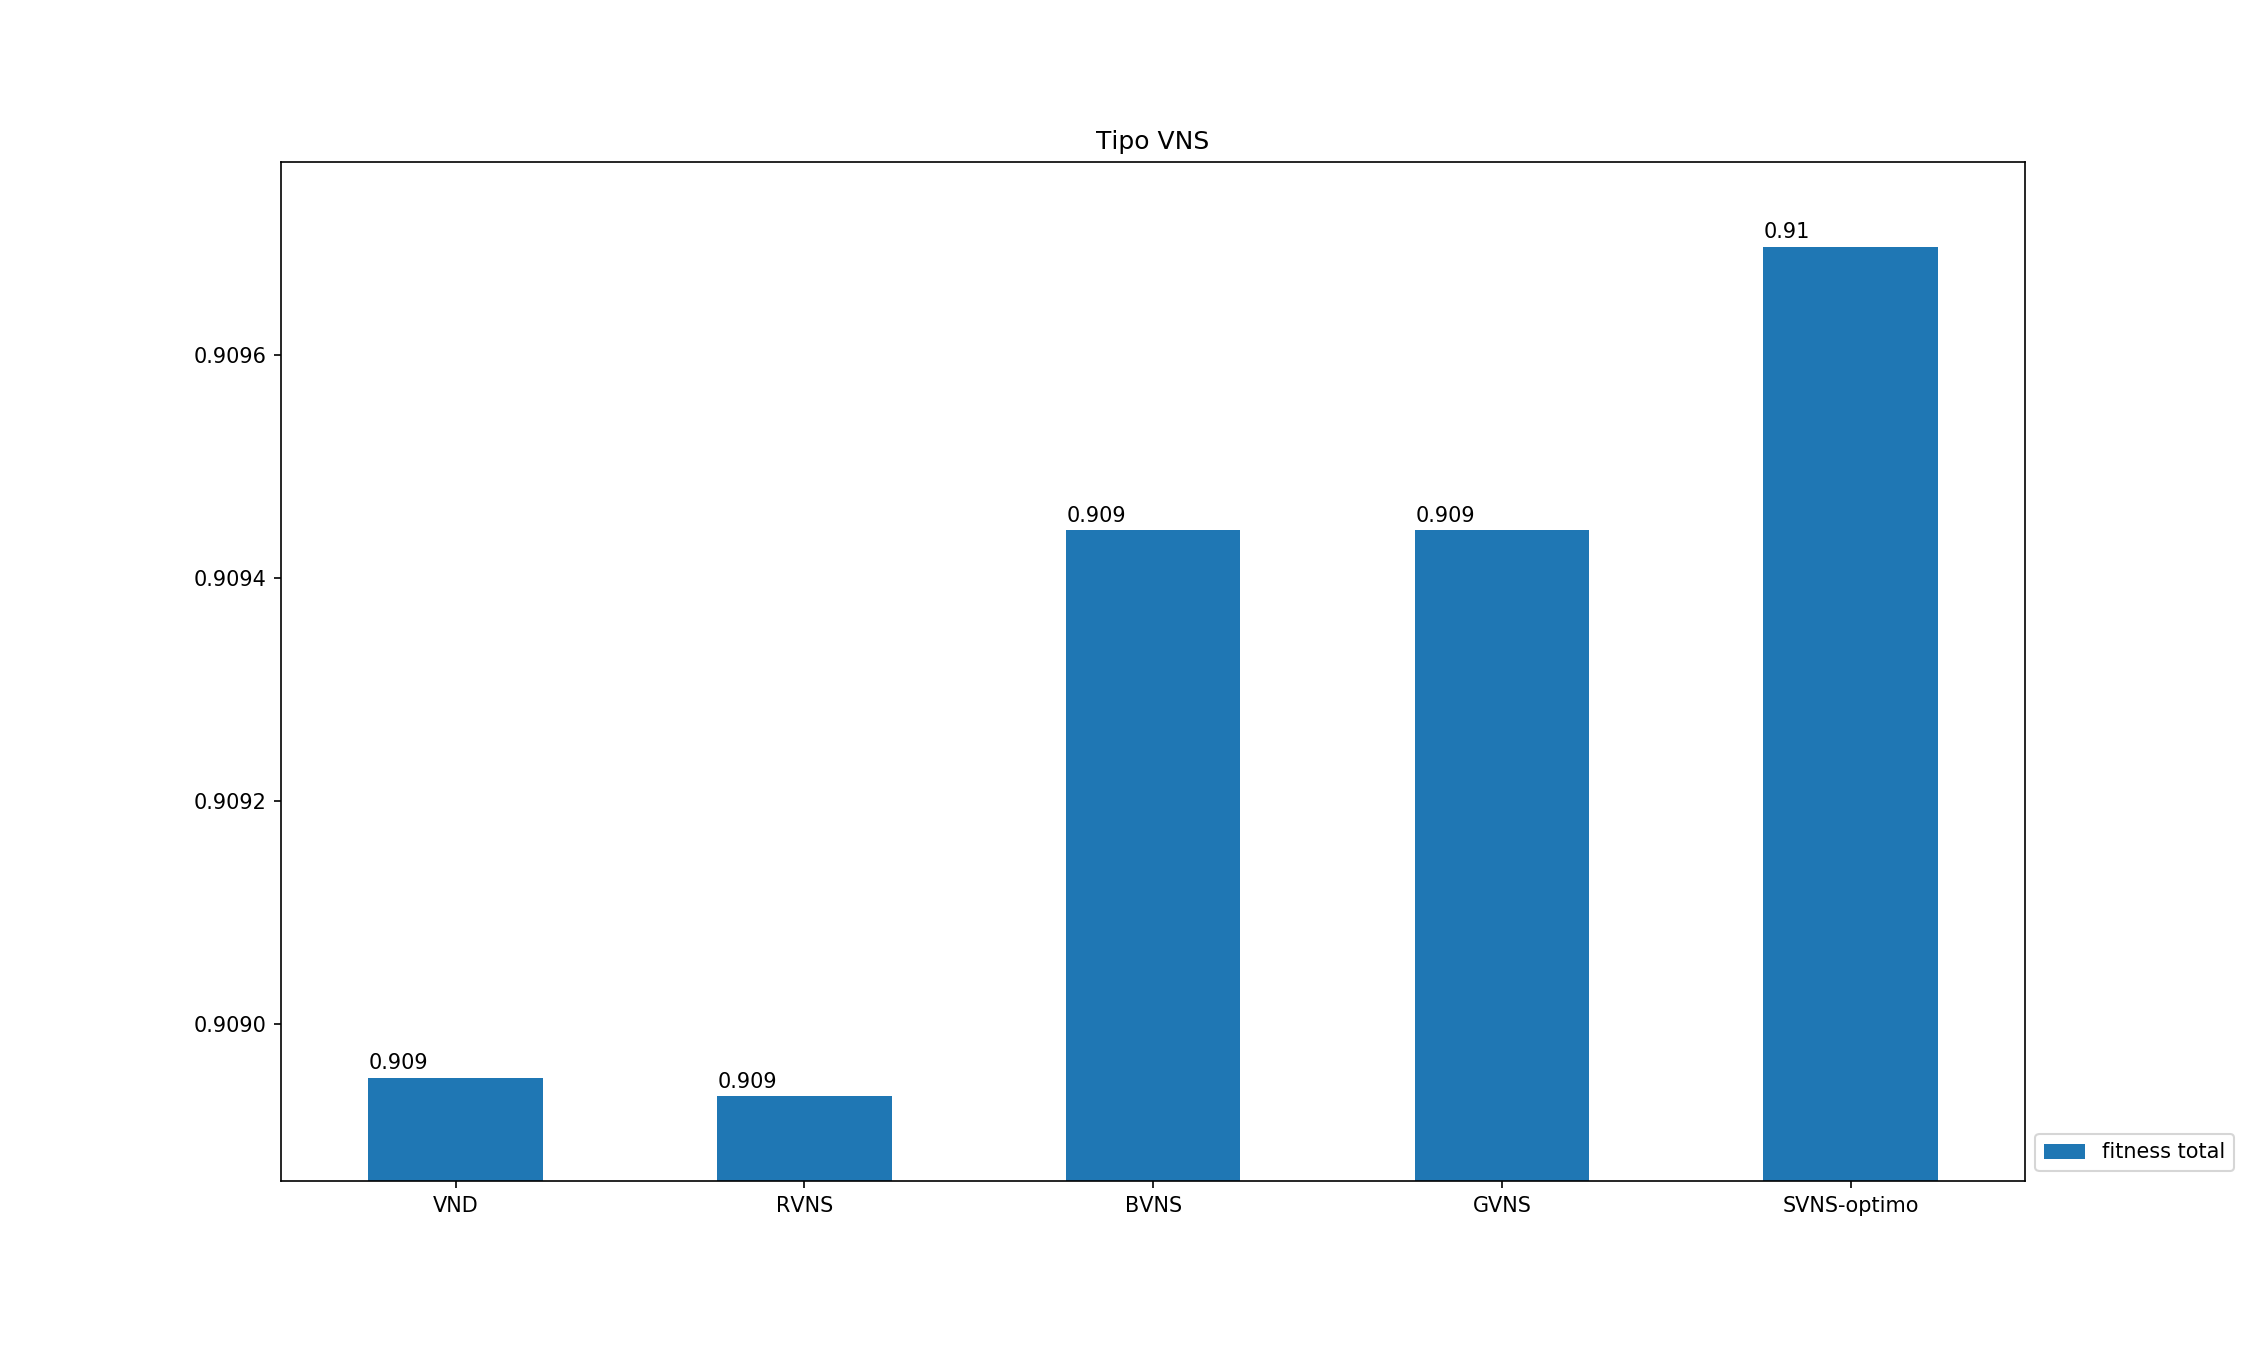
\includegraphics[width=\linewidth]{caso4-tipo-orden-tiempo}
	\caption{Variación del fitness según el tipo de VNS para el caso 4. Ordenado según el tiempo de ejecución de cada uno}
	\label{fig:caso4-tipo-orden-tiempo}
\end{figure}

Sin embargo, esta mejora se obtiene a costa de una mayor necesidad de tiempo de cómputo, con una diferencia de $31.2762$ segundos para el caso 4 del \textit{BVNS} frente al \textit{VND}. Sin duda hemos observado que el \textit{RVND} es el tipo de VNS que menos tiempo de cómputo requiere, pero suele ser el que peores resultados alcanza después del \textit{SVNS}. La \autoref{fig:caso4-tipo-orden-tiempo} ofrece adicionalmente un ranking donde nos muestra de forma ordenada los tipos de VNS que más tiempo consumen: como era de esperar, el \textit{SVNS} y el \textit{GVNS} son los más costosos, mientras que el \textit{VND} y \textit{RVNS} los que menos. Por su parte, el \textit{GVNS} y el \textit{BVNS} dan resultados que en la mayoría de los casos son muy similares entre sí, a excepción de en el caso 1 y el 3, donde los resultados son más dispares. En aquellos casos donde ha habido empate, se ha optado por usar la versión menos costosa computacionalmente, que es el \textit{BVNS}.

En la \autoref{fig:caso4y9comparativa-tipos-vnsiteracion} podemos observar la evolución por iteraciones de cada VNS, donde podemos apreciar cómo, a diferencia del resto, el \textit{SVNS} no es estrictamente creciente, aceptando soluciones peores. La línea \textit{SVNS-optimo} señala la mejor solución alcanzada hasta el momento por el \textit{SVNS}, que como podemos ver, no alcanza resultados tan buenos como los del resto. Cada ejecución termina cuando se alcanza la condición de parada del porcentaje mínimo de mejora. Además, el desempeño del \textit{BVNS} y el \textit{GVNS} es el mismo en ambos casos, aunque esto no siempre sucede en todas las iteraciones ni en todos los casos.

\begin{figure}
	\begin{subfigure}{\linewidth}
		\centering
		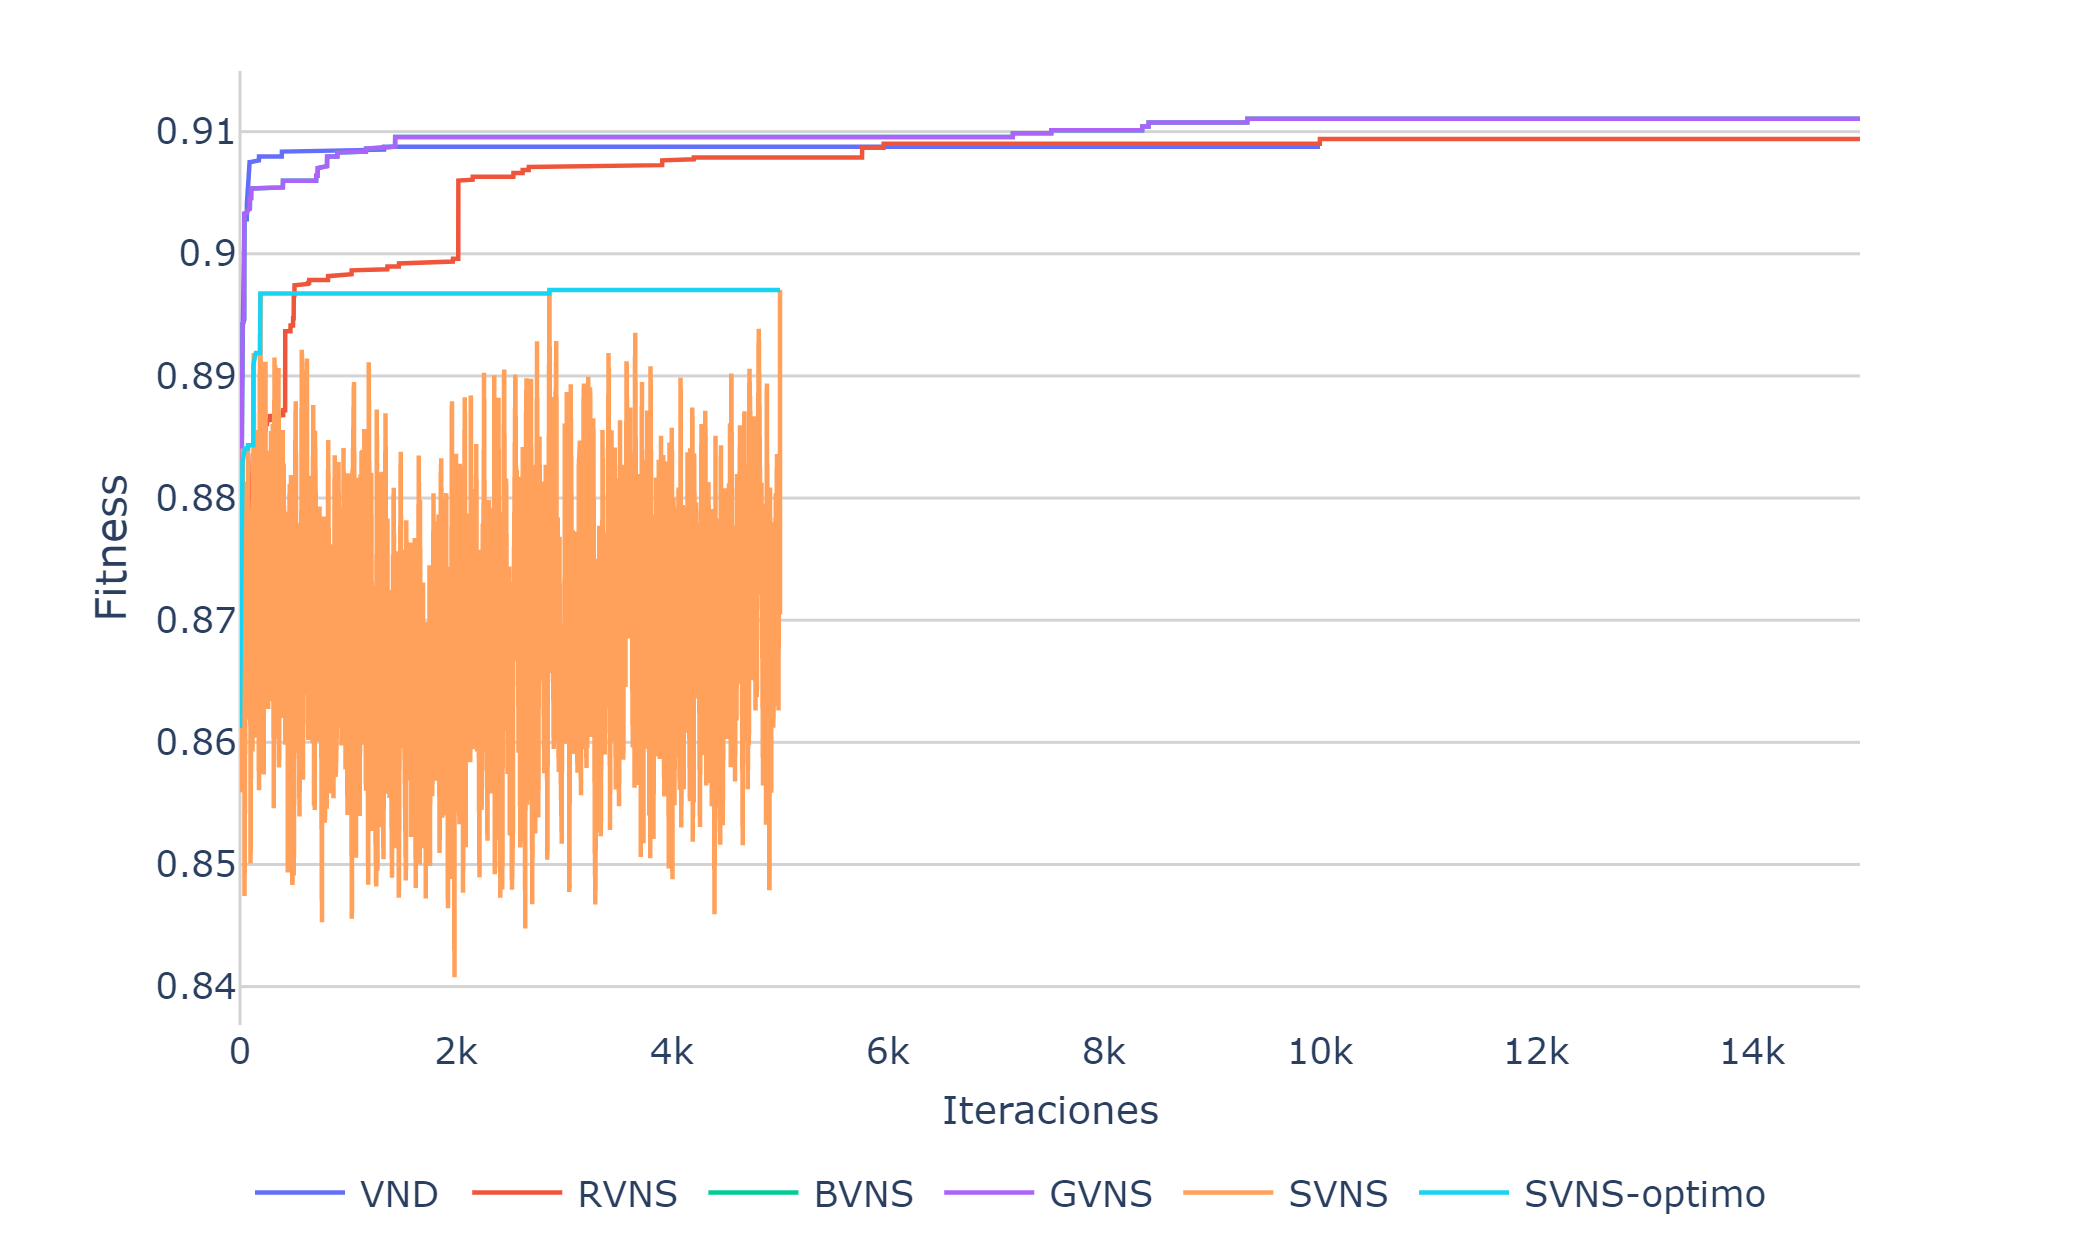
\includegraphics[width=\linewidth]{Caso4_comparativa-tipos-vns_iteracion}
		\caption{Caso 4}
		\label{fig:caso4comparativa-tipos-vnsiteracion}
	\end{subfigure}

	\begin{subfigure}{\linewidth}
		\centering
		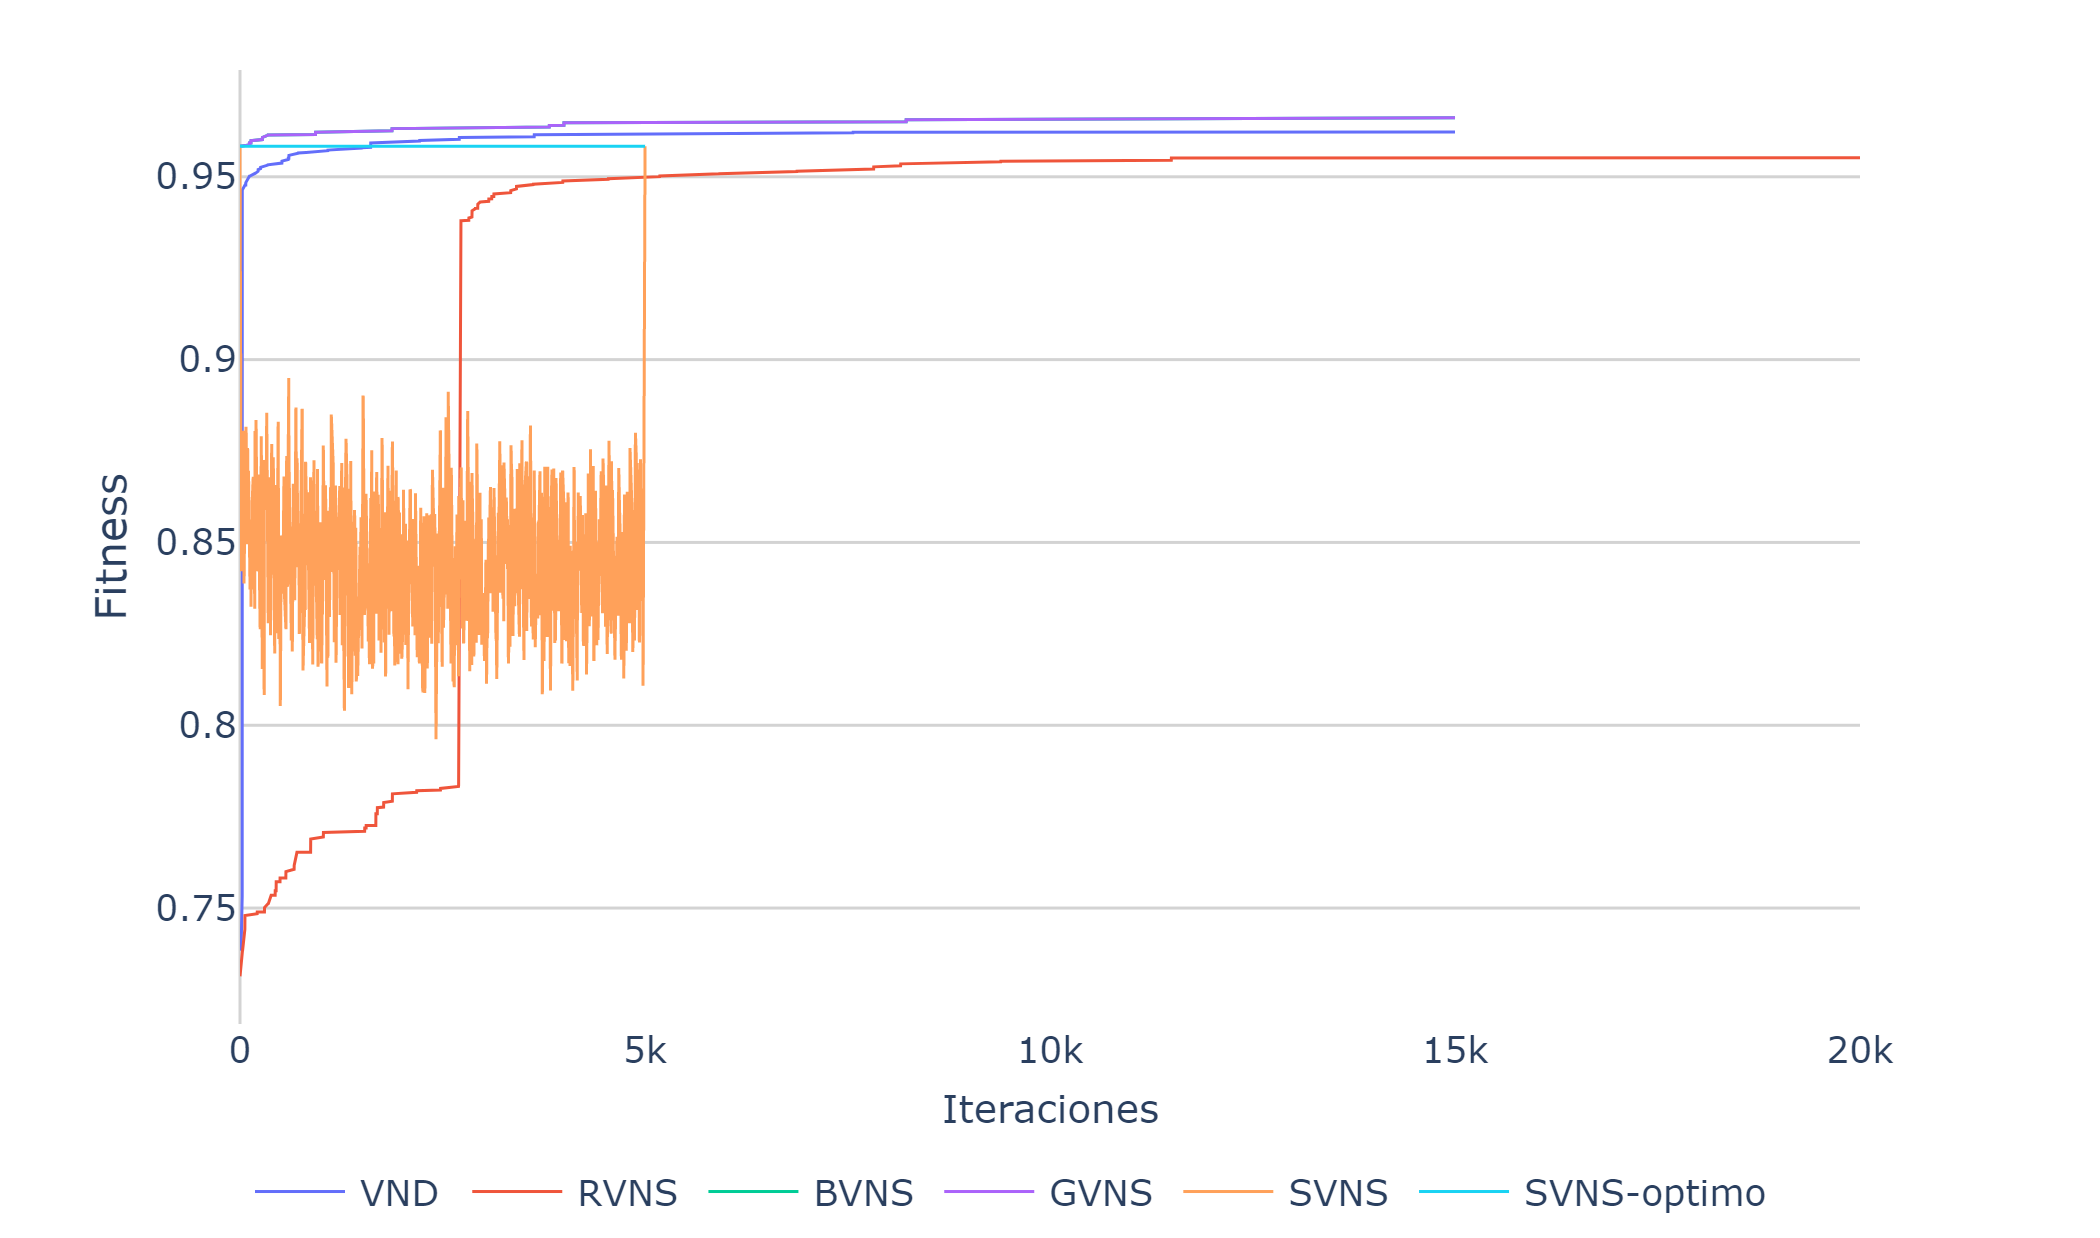
\includegraphics[width=\linewidth]{Caso9_comparativa-tipos-vns_iteracion}
		\caption{Caso 9}
		\label{fig:caso9comparativa-tipos-vnsiteracion}
	\end{subfigure}
	\caption{Evolución de cada \textbf{tipo de VNS} para una ejecución concreta del caso 4 y 9.}
	\label{fig:caso4y9comparativa-tipos-vnsiteracion}
\end{figure}

En cuanto al orden de los entornos, no hay una clara tendencia, pero sí observamos que el primero planteado, (a), es el menos efectivo, puesto que sus resultados son superados por otros. Por otro lado, la selección óptima de los mismos es claramente determinista, salvo en el caso 5 y 9. 
Una comparativa nos dice que la mejoría que aporta no es demasiado grande, del orden de una milésima (véase la \autoref{fig:caso5-naturaleza-entornos}) aunque para este caso concreto, con la opción probabilística, el número de restricciones incumplidas en la solución final es menos disperso que en la determinista, es decir, la diferencia entre una ejecución u otra no es tan grande como en el caso de la determinista. No obstante, para el resto de casos esta dispersión no sucede de una forma tan significativa.

\begin{figure}
	\centering
	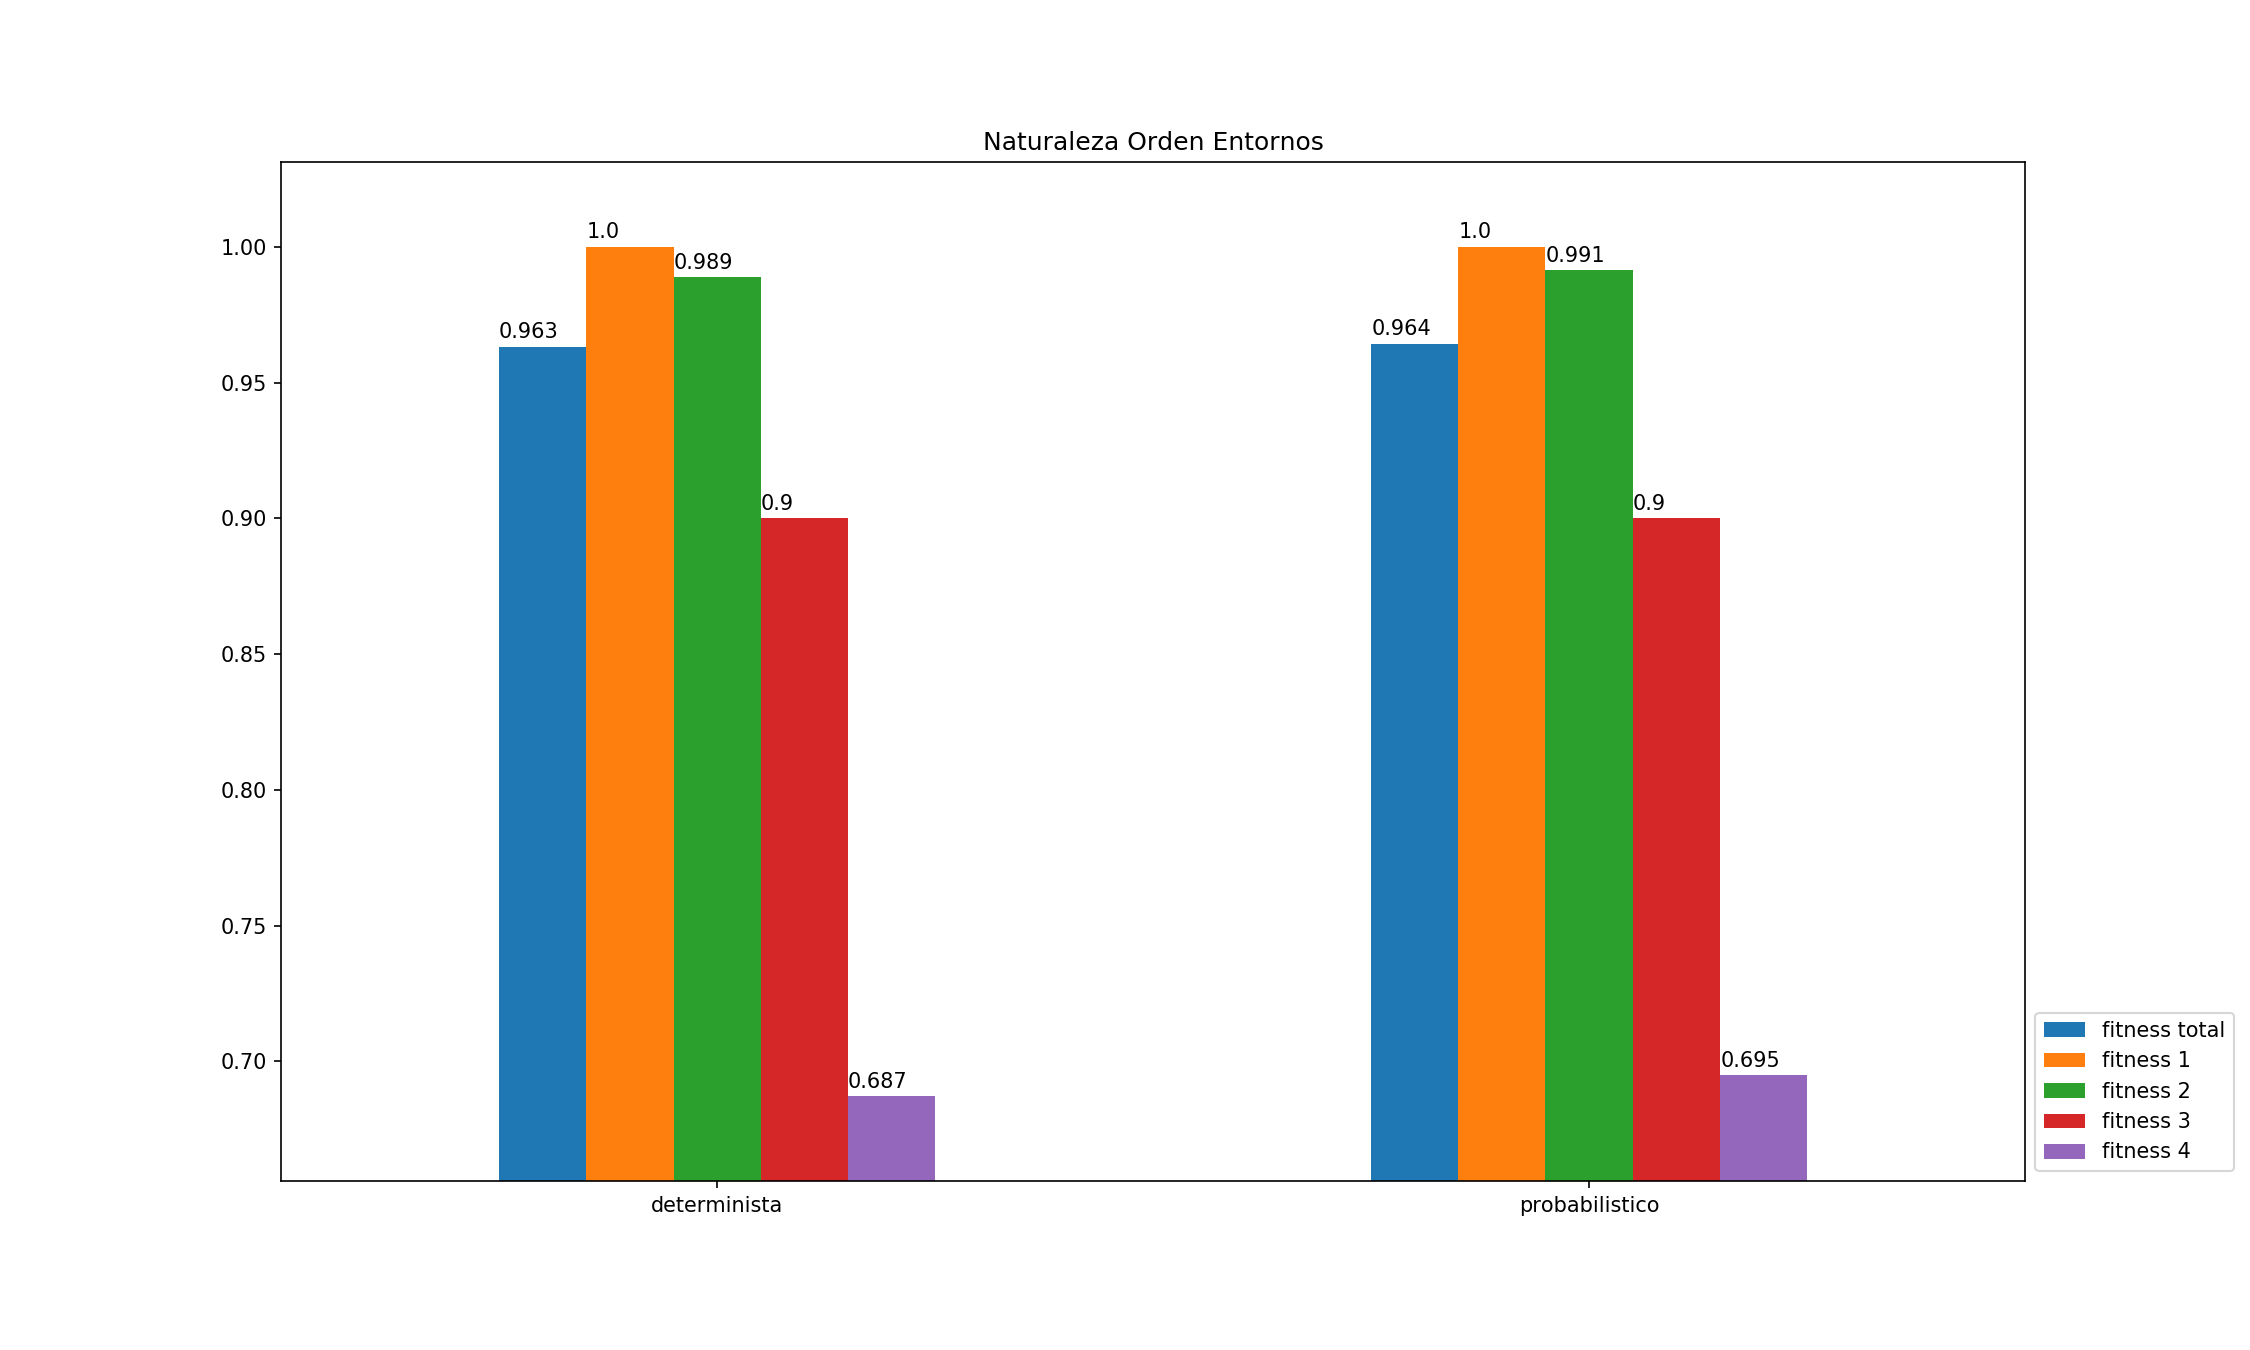
\includegraphics[width=1\linewidth]{caso5-naturaleza-entornos}
	\caption{Comparación desglosada por valor de cada objetivo para el \textbf{tipo de cambio de entorno} en el caso 5}
	\label{fig:caso5-naturaleza-entornos}
\end{figure}

En la \autoref{fig:caso4y9determinista-vs-probabilisticoiteracion} podemos observar la evolución de una ejecución, comparando el desempeño de sistema para cambios de entorno de tipo determinista y de tipo probabilístico, una vez seleccionados los parámetros óptimos relativos a este último. Se aprecia cómo, para el caso 9  (\autoref{fig:caso9determinista-vs-probabilisticoiteracion}), la diferencia es significativa: el probabilístico aporta lo suficiente como para ser utilizado. Sin embargo, para el caso 4~(\autoref{fig:caso4determinista-vs-probabilisticoiteracion}) el tipo de cambio de entornos determinista supera al probabilístico pero por muy poca diferencia.

\begin{figure}
	\begin{subfigure}{\linewidth}
		\centering
		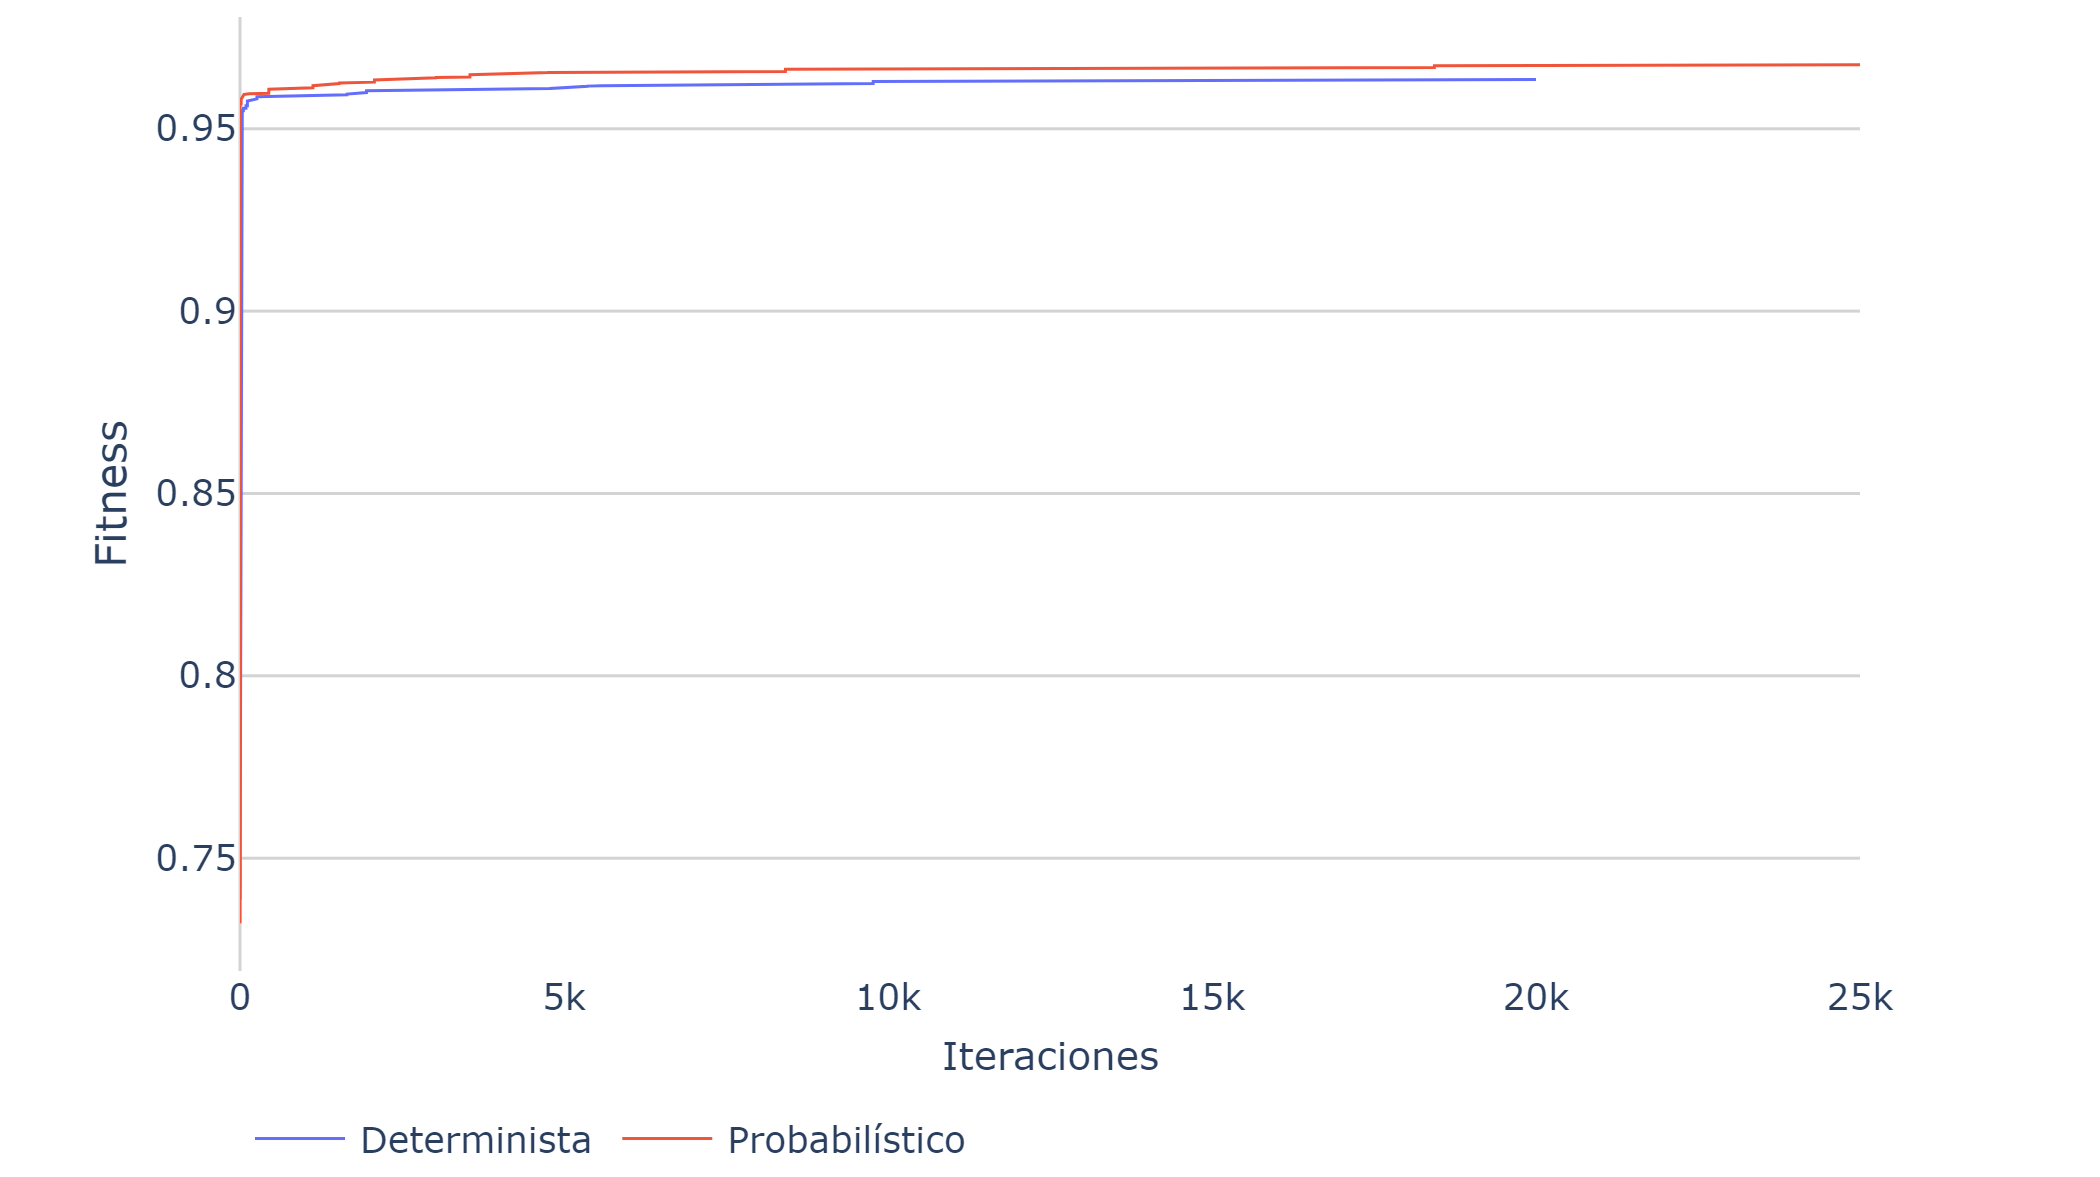
\includegraphics[width=1\linewidth]{Caso9_determinista-vs-probabilistico_iteracion}
		\caption{Caso 9}
		\label{fig:caso9determinista-vs-probabilisticoiteracion}
	\end{subfigure}

	\begin{subfigure}{\linewidth}
		\centering
		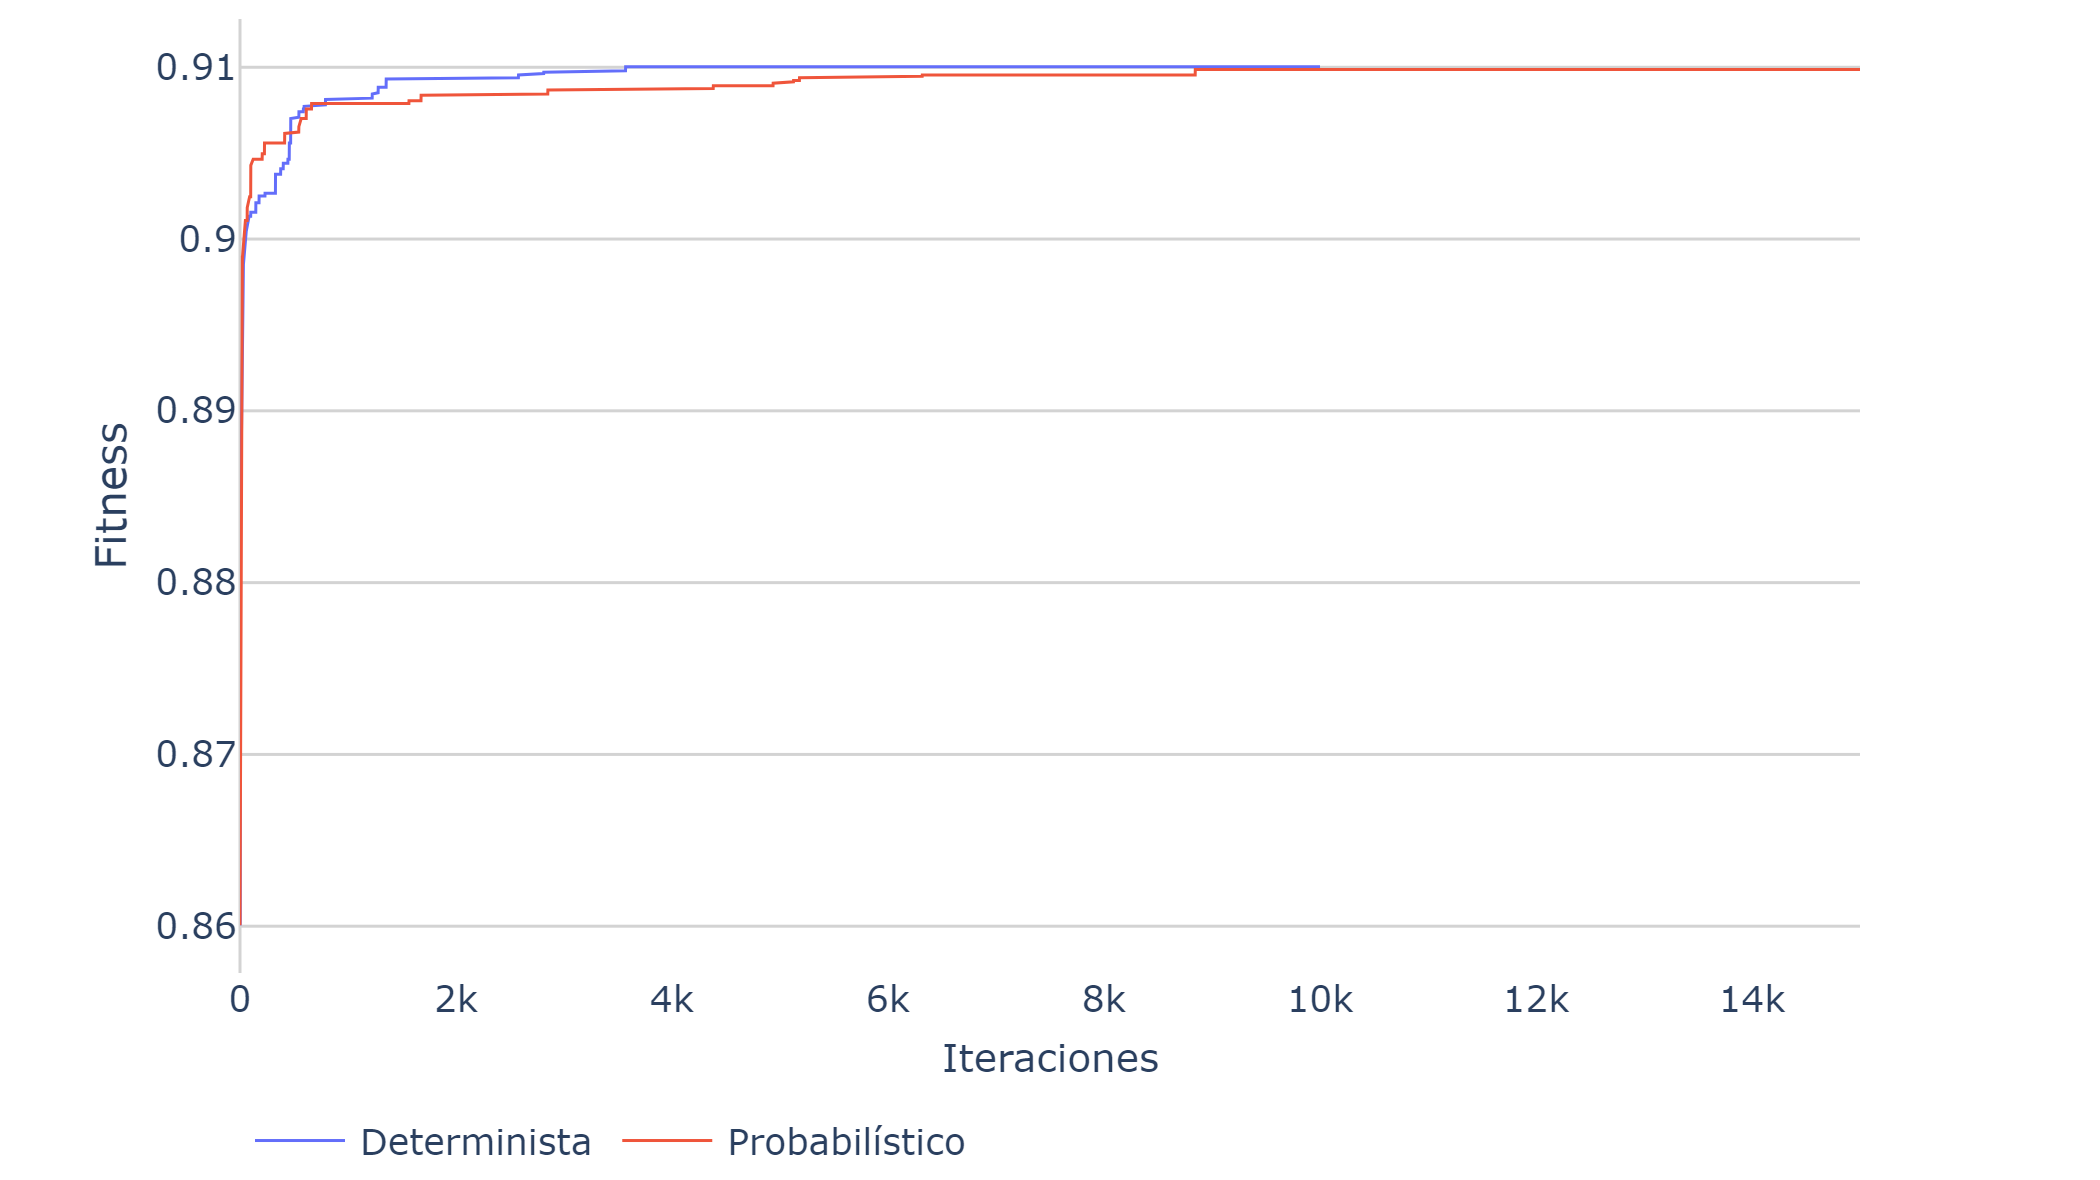
\includegraphics[width=1\linewidth]{Caso4_determinista-vs-probabilistico_iteracion}
		\caption{Caso 4}
		\label{fig:caso4determinista-vs-probabilisticoiteracion}
	\end{subfigure}
	\caption{Evolución del sistema para una ejecución concreta del caso 9 y 4 con \textbf{cambios de entorno} de tipo determinista o probabilístico.}
	\label{fig:caso4y9determinista-vs-probabilisticoiteracion}
\end{figure}


%Observamos que los parámetros óptimos que afectan a la modalidad probabilista de los entornos se adecuan al VNS en cuanto a que, por ejemplo emplear una probabilidad inicial de $0.7$ con una variación pequeña, en lugar de una probabilidad de 1, pues el número de iteraciones no es suficientemente grande como para que 

En cuanto a los demás parámetros, no hay diferencias importantes entre sí. El número de iteraciones que conforman el ciclo mínimo para comprobar la condición de parada se mueven entre $6\,000$ y $45\,000$. Para su elección fue tomado en cuenta no solo el valor de la función fitness, sino también el tiempo empleado, buscando un equilibrio entre ambos, pues como muestra la \autoref{fig:5:caso3-numero-iteraciones-para-comprobar-porcentaje-mejoria}, cuanto mayor es el número de iteraciones por ciclo, mayor es el valor de fitness hasta un punto en el que se estabiliza. No obstante hay ocasiones en las que el crecimiento es especialmente lento o más estable, como sucede en el caso 5 o 6. En esos casos, se ha optado por buscar el mencionado equilibrio, en el que el tiempo no fuese demasiado grande.

\begin{figure}
	\centering
	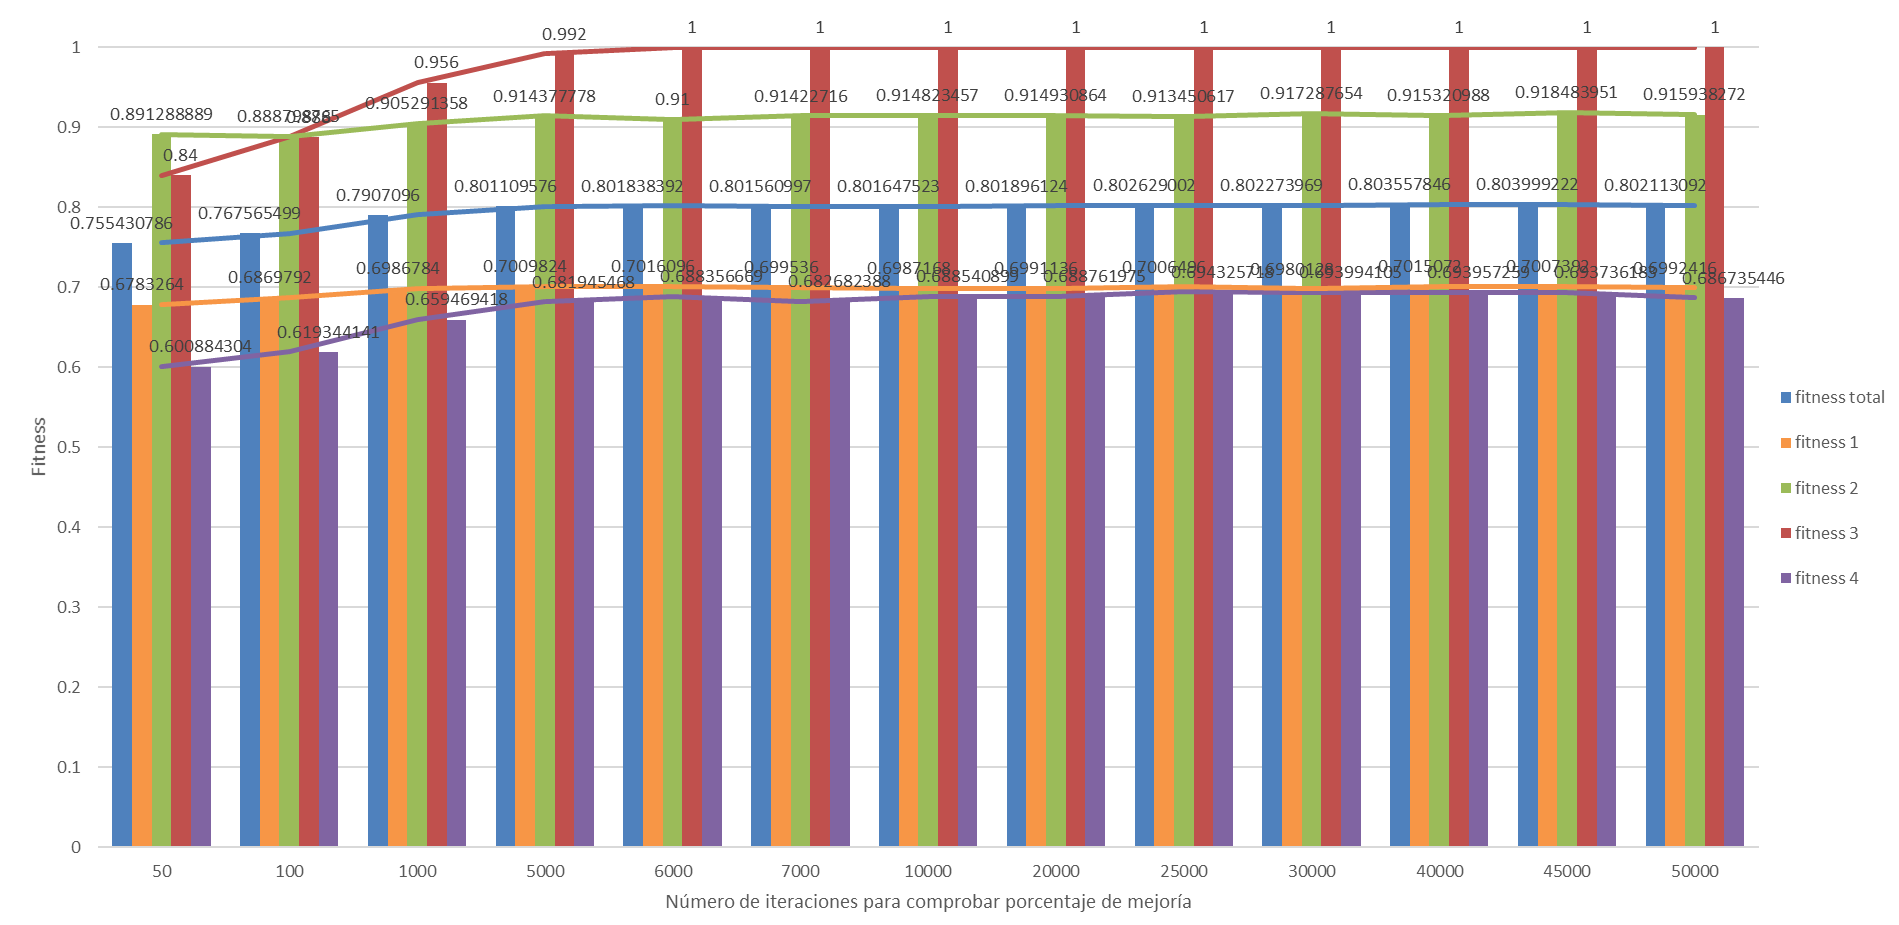
\includegraphics[width=\linewidth]{grafica-caso3-numero-iteraciones-para-comprobar-porcentaje-mejoria}
	\caption{Variación del valor de fitness desglosado para diferentes valores del parámetro del número de iteraciones para comprobar el porcentaje de mejoría del caso 3.}
	\label{fig:5:caso3-numero-iteraciones-para-comprobar-porcentaje-mejoria}
\end{figure}



La función de distancia aplicada para el \textit{SVNS} que mejores resultados alcanza es aquella que calcula el número de slots dispares entre ambas soluciones. Hemos observado que el valor del parámetro $\alpha$ óptimo oscila entre 0.5 y 2, y para tamaños superiores a 2, o bien deja de admitir soluciones peores, o bien se comporta de la misma forma que con otros valores inferiores. En la \autoref{fig:caso9comparativa-alphasiteracion0-5} podemos observar cómo se comporta la metaheurística \textit{SVNS} con diferentes $\alpha$ para el caso 9, si bien exploran de diferentes formas, no logran mejorar significativamente los resultados iniciales, aunque esto sí sucede aunque muy levemente, para el caso 3, como muestra la \autoref{fig:Caso3_comparativa-alphas_iteracion}.

\begin{figure}
	\begin{subfigure}{\linewidth}
	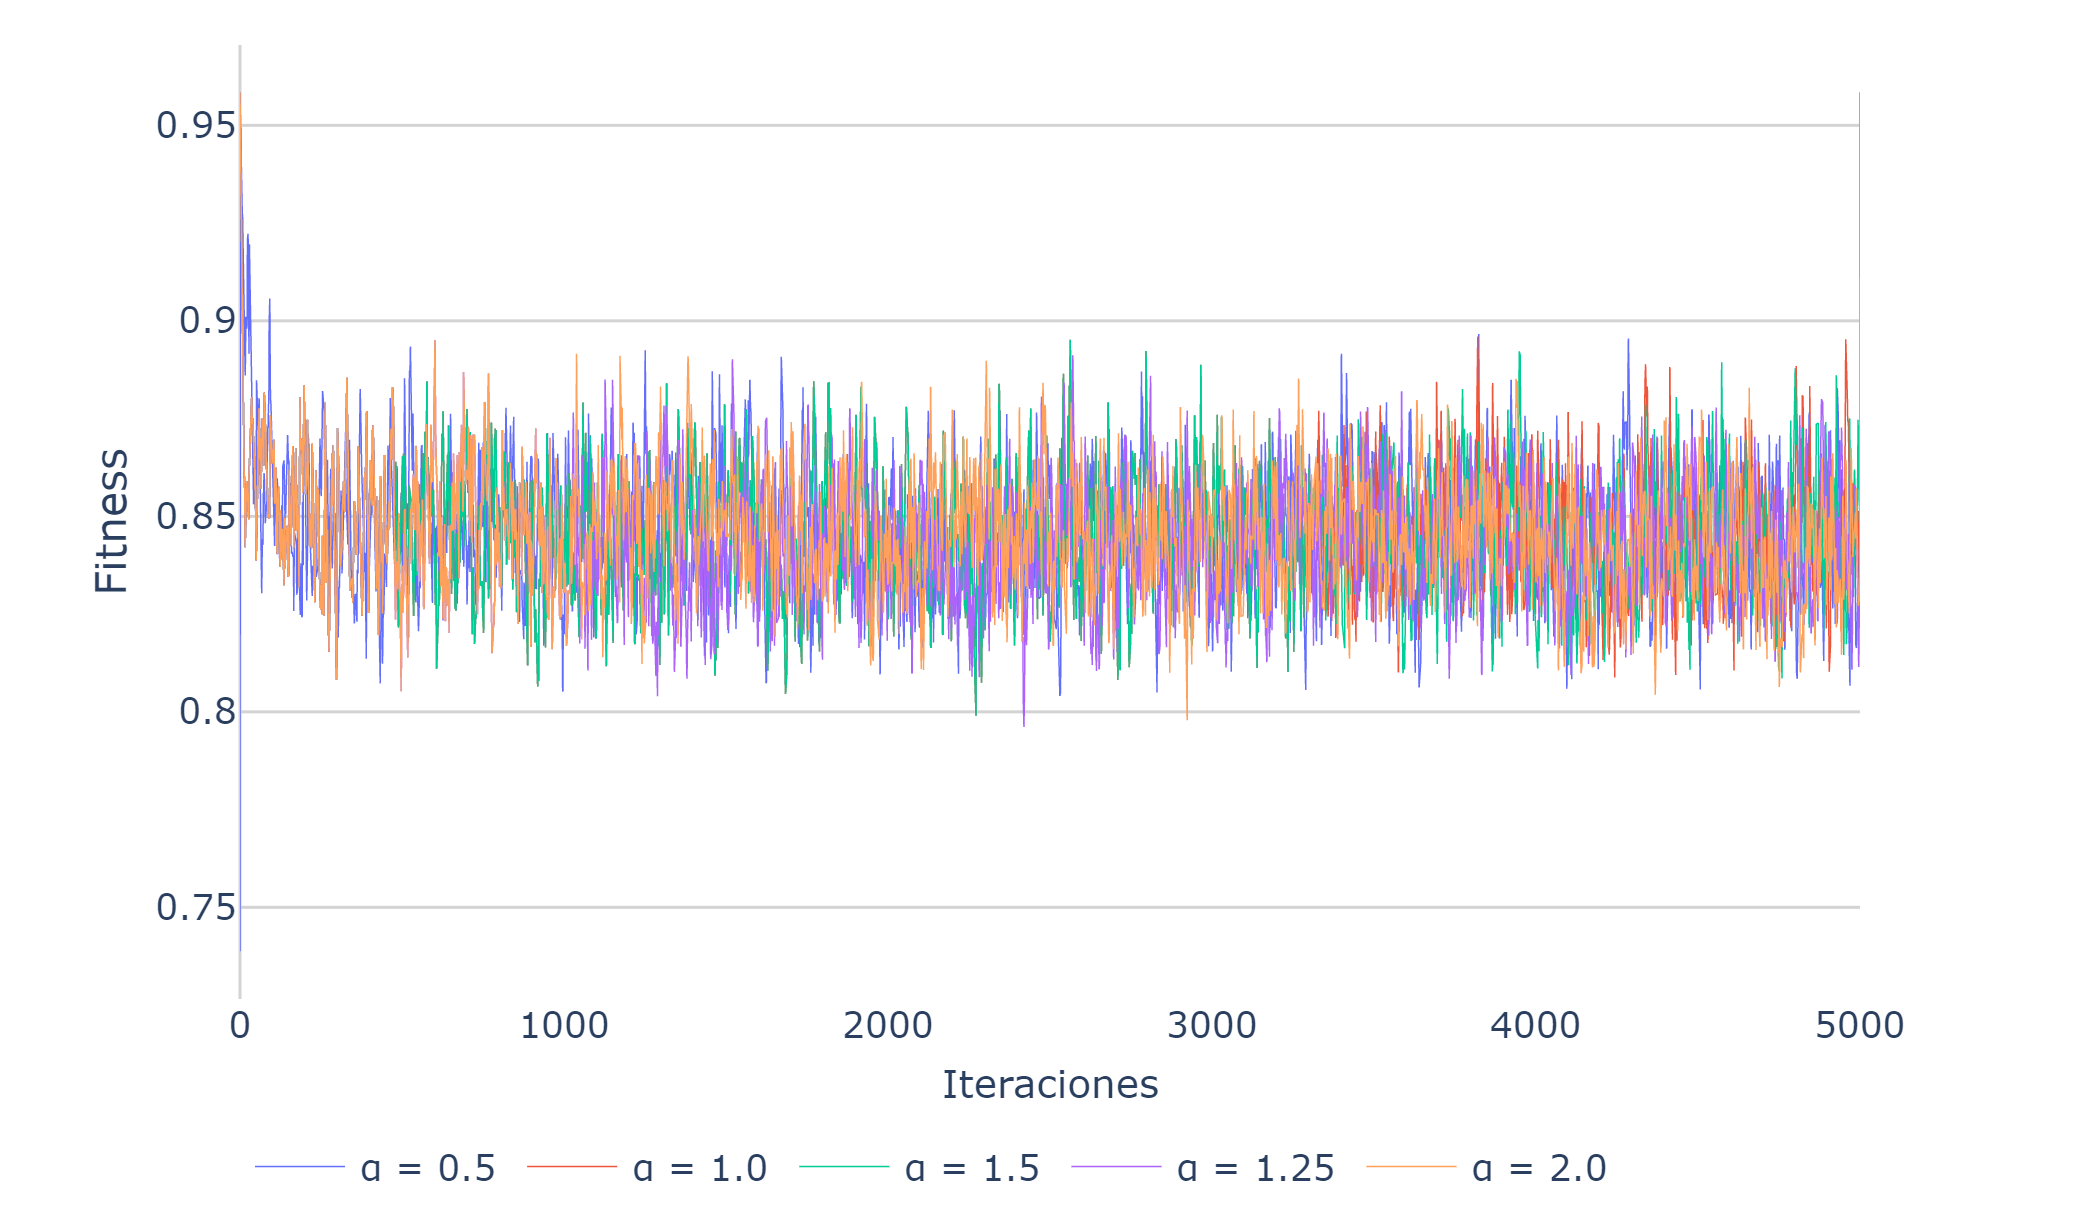
\includegraphics[width=\linewidth]{Caso9_comparativa-alphas_iteracion_0-5}
	\caption{Caso 9}
	\label{fig:caso9comparativa-alphasiteracion0-5}
	\centering
	\end{subfigure}

	\begin{subfigure}{\linewidth}
	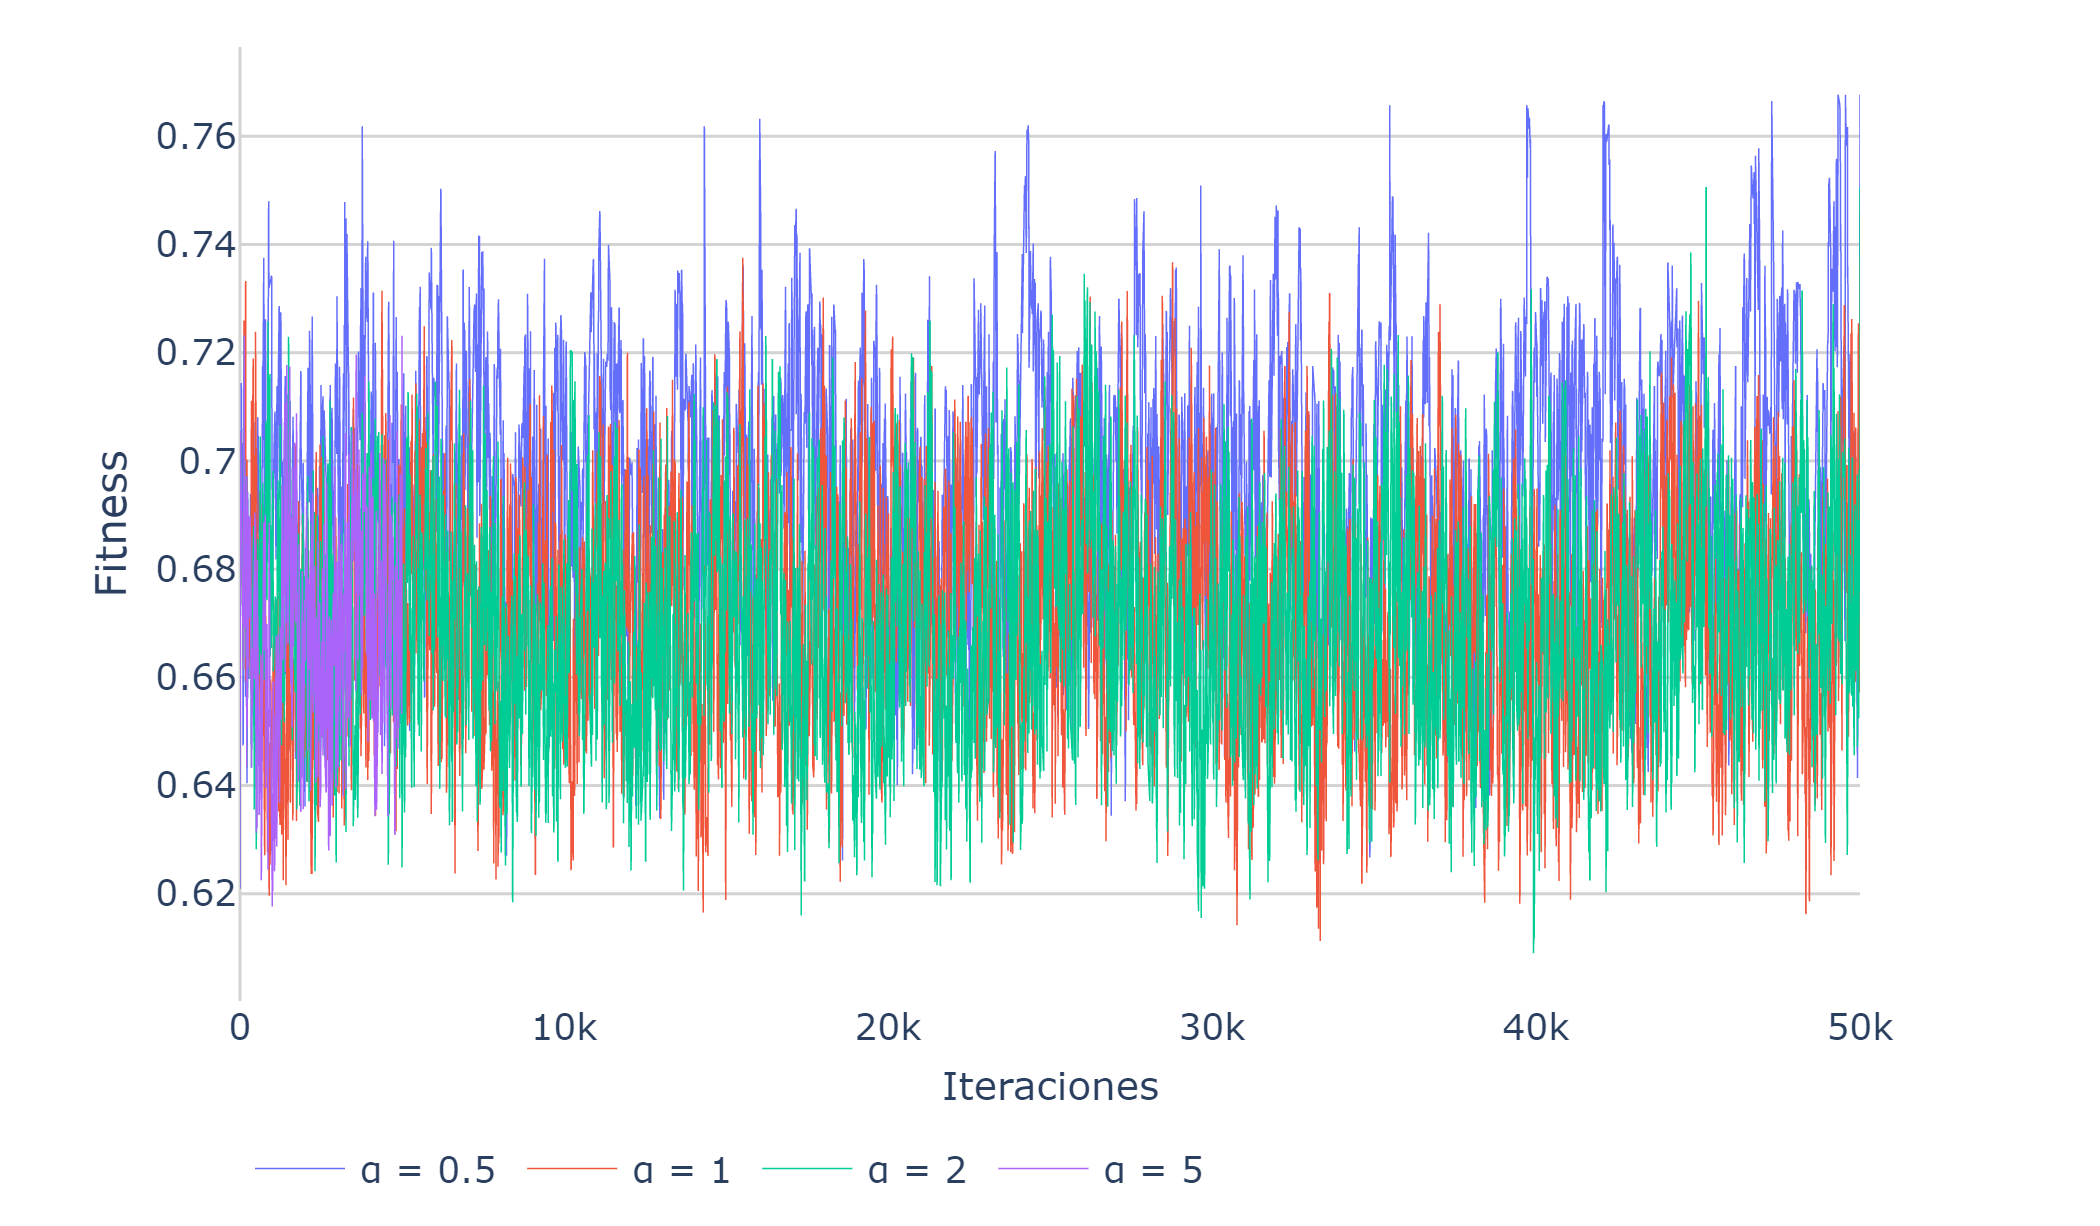
\includegraphics[width=\linewidth]{Caso3_comparativa-alphas_iteracion}
	\caption{Caso 3}
	\label{fig:Caso3_comparativa-alphas_iteracion}
	\centering
\end{subfigure}
	\caption{Evolución comparativa del desempeño del \textit{SVNS} con diferentes \textbf{alphas} para el caso 3 y el 9.}
\end{figure}

Las gráficas comparativas de los tipos de entornos, del tipo de VNS y de los distintos valores para el parámetro alpha incluidas en esta sección, junto con las demás del resto de los casos de prueba se encuentran disponibles y de manera interactiva en la web \url{https://sfv-tfm-recursos.000webhostapp.com/}.


%A continuación describiremos algunas de las observaciones en mayor profundidad.
%
%\subsubsection{Comparativa de Tipos de VNS}
%
%Como se ha mencionado anteriormente, se han obtenido dos tipos de VNS con resultados especialmente mejores: el \textit{VND} y el \textit{BVNS}. Por lo general, la diferencia no es realmente grande, a excepción del caso 5, donde la diferencia es de 5 centésimas, sin embargo, en los casos indicados, el aporte sigue siendo significativo al conjunto, y la diferencia de tiempo

\subsection{Comparación de metaheurísticas}

Una vez ajustados todos los parámetros para sacar el máximo rendimiento del sistema, podemos compararlo con otros, y en este caso, se ha hecho una comparación de resultados con la metaheurística \sa{} (SA), definida en la \autoref{sec:3:metaheurística}. Recuérdese que se trata de la metaheurística empleada para el desarrollo del sistema \legacy{} y que fue adaptada a las nuevas condiciones y restricciones del sistema implementado en este TFM.

Es importante destacar en este punto, que la \faseuno{}, de inicialización, es la misma en ambas metaheurísticas. La única diferencia entre unas ejecuciones u otras está únicamente en la \fasedos{}, es decir, la metaheurística en sí.

La \autoref{table:comparativa-sa-vns-porcentaje} y \ref{table:comparativa-sa-vns-tiempo} recopilan los resultados medios (de 10 ejecuciones distintas) para ambas metaheurísticas, variando la condición de parada: porcentaje mínimo de mejora y tiempo máximo. El porcentaje de cada caso y de cada metaheurística empleados son aquellos con los que se alcanzan los resultados óptimos, por lo que dependen de las características tanto de las metaheurísticas como de los propios casos, por lo que no es invariante, a diferencia de la condición de parada por tiempo, que se optó por emplear un tiempo exacto de 10 minutos, de manera que forzamos a las metaheurísticas a ejecutar ese tiempo. 

Encontramos casos donde, tanto en VNS como en SA, empleando la condición de parada optimizada al porcentaje mínimo de mejora, terminaría su ejecución en un tiempo menor de los 10 minutos, pero también tenemos casos en los que sucede lo opuesto. Por ejemplo, el caso 5 nos ocupa un tiempo de ejecución de 25 minutos, que al emplear como condición de parada el tiempo, se está limitando su tiempo de ejecución y por ende es natural que los resultados sean peores. Con la mayoría de los casos sucede lo contrario: tardan menos de los 10 minutos, y como vemos al comparar ambas tablas, en algunos casos hay una pequeña mejoría, pero no nos parece suficiente a cambio del tiempo empleado.

\begin{table}
	\centering
	\caption{Tabla comparativa con condición de parada establecida únicamente por porcentaje mínimo de mejora}
	\label{table:comparativa-sa-vns-porcentaje}
	\resizebox{\textwidth}{!}{%
		\begin{tabular}{cccccccccc}
			\hline
			\multicolumn{10}{c}{}                                                                                                                                                                                                                                                                                                                                                                                                                                                                   \\
			\multicolumn{10}{c}{Condición de Parada: Porcentaje de mejora}                                                                                                                                                                                                                                                                                                                                                                                                                          \\
			\multicolumn{10}{c}{}                                                                                                                                                                                                                                                                                                                                                                                                                                                                   \\ \cline{3-10} 
			&                               & \begin{tabular}[c]{@{}c@{}}Restricciones \\ incumplidas\end{tabular} & \begin{tabular}[c]{@{}c@{}}Número de \\ controladores\end{tabular} & \begin{tabular}[c]{@{}c@{}}Fitness\\ total\end{tabular} & f1                            & f2                            & f3                            & f4                            & Tiempo (min) \\ \cline{3-10} 
			\multicolumn{10}{c}{}                                                                                                                                                                                                                                                                                                                                                                                                                                                                   \\
			\multicolumn{1}{c|}{}                      & {\color[HTML]{003532} Caso 1} & {\color[HTML]{003532} 58.13}                                         & {\color[HTML]{9A0000} \textbf{25}}                                 & {\color[HTML]{9A0000} \textbf{0.7117}}                  & {\color[HTML]{003532} 0.7229} & {\color[HTML]{003532} 0.8686} & {\color[HTML]{003532} 0.4400} & {\color[HTML]{003532} 0.5877} & {\color[HTML]{003532} 21.09}                                         \\
			\multicolumn{1}{c|}{}                      & Caso 3                        & 65.07                                                                & 25                                                                 & 0.6262                                                  & 0.5984                        & 0.8465                        & 0.3600                        & 0.5412                        & 21.5                                                                 \\
			\multicolumn{1}{c|}{}                      & {\color[HTML]{003532} Caso 4} & {\color[HTML]{003532} 2.00}                                          & {\color[HTML]{003532} 19}                                          & {\color[HTML]{003532} 0.9111}                           & {\color[HTML]{003532} 1.0000} & {\color[HTML]{003532} 0.9941} & {\color[HTML]{003532} 0.4737} & {\color[HTML]{003532} 0.8598} & {\color[HTML]{003532} 7.54}                                          \\
			\multicolumn{1}{c|}{}                      & Caso 5                        & 0.00                                                                 & 20                                                                 & 0.9432                                                  & 1.0000                        & 1.0000                        & 0.8000                        & 0.5539                        & 4.76                                                                 \\
			\multicolumn{1}{c|}{}                      & {\color[HTML]{003532} Caso 6} & {\color[HTML]{003532} 5.00}                                          & {\color[HTML]{003532} 19}                                          & {\color[HTML]{003532} 0.9489}                           & {\color[HTML]{003532} 1.0000} & {\color[HTML]{003532} 0.9795} & {\color[HTML]{003532} 0.7894} & {\color[HTML]{003532} 0.7675} & {\color[HTML]{003532} 9.68}                                          \\
			\multicolumn{1}{c|}{}                      & Caso 7                        & 27.50                                                                & {\color[HTML]{9A0000} \textbf{28}}                                 & {\color[HTML]{9A0000} \textbf{0.6146}}                  & 0.5221                        & 0.9491                        & 0.3000                        & 0.6972                        & 61.6                                                                 \\
			\multicolumn{1}{c|}{}                      & {\color[HTML]{003532} Caso 8} & {\color[HTML]{003532} 2.00}                                          & {\color[HTML]{003532} 22}                                          & {\color[HTML]{003532} 0.9684}                           & {\color[HTML]{003532} 1.0000} & {\color[HTML]{003532} 0.9949} & {\color[HTML]{003532} 0.9090} & {\color[HTML]{003532} 0.7238} & {\color[HTML]{003532} 10.31}                                         \\
			\multicolumn{1}{c|}{\multirow{-8}{*}{SA}}  & Caso 9                        & 0.00                                                                 & 23                                                                 & 0.9711                                                  & 1.0000                        & 1.0000                        & 0.9130                        & 0.7360                        & 6.01                                                                 \\
			\multicolumn{10}{c}{}                                                                                                                                                                                                                                                                                                                                                                                                                                                                   \\
			\multicolumn{1}{c|}{}                      & {\color[HTML]{003532} Caso 1} & {\color[HTML]{003532} 12.8183}                                       & {\color[HTML]{9A0000} \textbf{24}}                                 & {\color[HTML]{9A0000} \textbf{0.9718}}                  & {\color[HTML]{003532} 1.0000} & {\color[HTML]{003532} 0.9703} & {\color[HTML]{003532} 0.8333} & {\color[HTML]{003532} 0.6632} & {\color[HTML]{003532} 6.1894}                                        \\
			\multicolumn{1}{c|}{}                      & Caso 3                        & 37.1767                                                              & 25                                                                 & 0.8041                                                  & 0.7015                        & 0.9174                        & 1.0000                        & 0.6933                        & 7.2020                                                               \\
			\multicolumn{1}{c|}{}                      & {\color[HTML]{003532} Caso 4} & {\color[HTML]{003532} 2.0000}                                        & {\color[HTML]{003532} 19}                                          & {\color[HTML]{003532} 0.9105}                           & {\color[HTML]{003532} 1.0000} & {\color[HTML]{003532} 0.9942} & {\color[HTML]{003532} 0.4737} & {\color[HTML]{003532} 0.8505} & {\color[HTML]{003532} 2.8527}                                        \\
			\multicolumn{1}{c|}{}                      & Caso 5                        & 1.8000                                                               & 20                                                                 & 0.9668                                                  & 1.0000                        & 0.9950                        & 0.9000                        & 0.7194                        & 25.7926                                                              \\
			\multicolumn{1}{c|}{}                      & {\color[HTML]{003532} Caso 6} & {\color[HTML]{003532} 6.6200}                                        & {\color[HTML]{003532} 19}                                          & {\color[HTML]{003532} 0.9467}                           & {\color[HTML]{003532} 1.0000} & {\color[HTML]{003532} 0.9806} & {\color[HTML]{003532} 0.7895} & {\color[HTML]{003532} 0.7257} & {\color[HTML]{003532} 0.7935}                                        \\
			\multicolumn{1}{c|}{}                      & Caso 7                        & 5.2000                                                               & {\color[HTML]{9A0000} \textbf{26}}                                 & {\color[HTML]{9A0000} \textbf{0.9335}}                  & 1.0000                        & 0.9889                        & 0.6923                        & 0.7102                        & 7.5845                                                               \\
			\multicolumn{1}{c|}{}                      & {\color[HTML]{003532} Caso 8} & {\color[HTML]{003532} 4.4000}                                        & {\color[HTML]{003532} 22}                                          & {\color[HTML]{003532} 0.9651}                           & {\color[HTML]{003532} 1.0000} & {\color[HTML]{003532} 0.9889} & {\color[HTML]{003532} 0.9091} & {\color[HTML]{003532} 0.6953} & {\color[HTML]{003532} 22.5359}                                       \\
			\multicolumn{1}{c|}{\multirow{-8}{*}{VNS}} & Caso 9                        & 4.0400                                                               & 23                                                                 & 0.9659                                                  & 1.0000                        & 0.9902                        & 0.9130                        & 0.6923                        & 9.3945                                                               \\
			\multicolumn{10}{c}{}                                                                                                                                                                                                                                                                                                                                                                                                                                                                   \\ \hline
		\end{tabular}%
	}
\end{table}


\begin{table}
	\centering
	\caption{Tabla comparativa con condición de parada establecida que limita el tiempo de ejecución a 10 minutos}
	\label{table:comparativa-sa-vns-tiempo}
	\resizebox{\textwidth}{!}{%
		\begin{tabular}{cccccccccc}
			\hline
			\multicolumn{10}{c}{}                                                                                                                                                                                                                                                                                                                                                                                                                                                                   \\
			\multicolumn{10}{c}{Condición de Parada: Tiempo de ejecución}                                                                                                                                                                                                                                                                                                                                                                                                                           \\
			\multicolumn{10}{c}{}                                                                                                                                                                                                                                                                                                                                                                                                                                                                   \\ \cline{3-10} 
			&                               & \begin{tabular}[c]{@{}c@{}}Restricciones \\ incumplidas\end{tabular} & \begin{tabular}[c]{@{}c@{}}Número de \\ controladores\end{tabular} & \begin{tabular}[c]{@{}c@{}}Fitness\\ total\end{tabular} & f1                            & f2                            & f3                            & f4                            & Tiempo (min) \\ \cline{3-10} 
			\multicolumn{10}{c}{}                                                                                                                                                                                                                                                                                                                                                                                                                                                                   \\
			\multicolumn{1}{c|}{}                      & {\color[HTML]{003532} Caso 1} & {\color[HTML]{003532} 6.00}                                          & {\color[HTML]{9A0000} \textbf{27}}                                 & {\color[HTML]{9A0000} \textbf{0.6095}}                  & {\color[HTML]{003532} 0.4944} & {\color[HTML]{003532} 0.9877} & {\color[HTML]{003532} 0.3333} & {\color[HTML]{003532} 0.5946} & {\color[HTML]{003532} 10}                                            \\
			\multicolumn{1}{c|}{}                      & Caso 3                        & 31.27                                                                & 25                                                                 & 0.7076                                                  & 0.6591                        & 0.9260                        & 0.5200                        & 0.6150                        & 10                                                                   \\
			\multicolumn{1}{c|}{}                      & {\color[HTML]{003532} Caso 4} & {\color[HTML]{003532} 2.00}                                          & {\color[HTML]{003532} 19}                                          & {\color[HTML]{003532} 0.9107}                           & {\color[HTML]{003532} 1.0000} & {\color[HTML]{003532} 0.9941} & {\color[HTML]{003532} 0.4737} & {\color[HTML]{003532} 0.8532} & {\color[HTML]{003532} 10}                                            \\
			\multicolumn{1}{c|}{}                      & Caso 5                        & 0.00                                                                 & 20                                                                 & 0.9599                                                  & 1.0000                        & 1.0000                        & 0.9000                        & 0.5825                        & 10                                                                   \\
			\multicolumn{1}{c|}{}                      & {\color[HTML]{003532} Caso 6} & {\color[HTML]{003532} 4.00}                                          & {\color[HTML]{003532} 19}                                          & {\color[HTML]{003532} 0.9483}                           & {\color[HTML]{003532} 1.0000} & {\color[HTML]{003532} 0.9854} & {\color[HTML]{003532} 0.7895} & {\color[HTML]{003532} 0.7300} & {\color[HTML]{003532} 10}                                            \\
			\multicolumn{1}{c|}{}                      & Caso 7                        & 27.50                                                                & {\color[HTML]{9A0000} \textbf{28}}                                 & {\color[HTML]{9A0000} \textbf{0.6146}}                  & 0.5221                        & 0.9491                        & 0.3000                        & 0.6972                        & 10                                                                   \\
			\multicolumn{1}{c|}{}                      & {\color[HTML]{003532} Caso 8} & {\color[HTML]{003532} 3.00}                                          & {\color[HTML]{003532} 22}                                          & {\color[HTML]{003532} 0.9702}                           & {\color[HTML]{003532} 1.0000} & {\color[HTML]{003532} 0.9924} & {\color[HTML]{003532} 0.9000} & {\color[HTML]{003532} 0.7644} & {\color[HTML]{003532} 10}                                            \\
			\multicolumn{1}{c|}{\multirow{-8}{*}{SA}}  & Caso 9                        & 3.00                                                                 & 23                                                                 & 0.9689                                                  & 1.0000                        & 0.9928                        & 0.9130                        & 0.7312                        & 10                                                                   \\
			\multicolumn{10}{c}{}                                                                                                                                                                                                                                                                                                                                                                                                                                                                   \\
			\multicolumn{1}{c|}{}                      & {\color[HTML]{003532} Caso 1} & {\color[HTML]{003532} 11.7111}                                       & {\color[HTML]{9A0000} \textbf{24}}                                 & {\color[HTML]{9A0000} \textbf{0.9721}}                  & {\color[HTML]{003532} 1.0000} & {\color[HTML]{003532} 0.9729} & {\color[HTML]{003532} 0.8333} & {\color[HTML]{003532} 0.6575} & {\color[HTML]{003532} 10}                                            \\
			\multicolumn{1}{c|}{}                      & Caso 3                        & 37.8778                                                              & 25                                                                 & 0.8016                                                  & 0.6981                        & 0.9158                        & 1.0000                        & 0.6894                        & 10                                                                   \\
			\multicolumn{1}{c|}{}                      & {\color[HTML]{003532} Caso 4} & {\color[HTML]{003532} 2.0000}                                        & {\color[HTML]{003532} 19}                                          & {\color[HTML]{003532} 0.9107}                           & {\color[HTML]{003532} 1.0000} & {\color[HTML]{003532} 0.9942} & {\color[HTML]{003532} 0.4737} & {\color[HTML]{003532} 0.8532} & {\color[HTML]{003532} 10}                                            \\
			\multicolumn{1}{c|}{}                      & Caso 5                        & 1.7500                                                               & 20                                                                 & 0.9659                                                  & 1.0000                        & 0.9951                        & 0.9000                        & 0.7033                        & 10                                                                   \\
			\multicolumn{1}{c|}{}                      & {\color[HTML]{003532} Caso 6} & {\color[HTML]{003532} 9.3500}                                        & {\color[HTML]{003532} 19}                                          & {\color[HTML]{003532} 0.9436}                           & {\color[HTML]{003532} 1.0000} & {\color[HTML]{003532} 0.9727} & {\color[HTML]{003532} 0.7895} & {\color[HTML]{003532} 0.7086} & {\color[HTML]{003532} 10}                                            \\
			\multicolumn{1}{c|}{}                      & Caso 7                        & 4.8101                                                               & {\color[HTML]{9A0000} \textbf{26}}                                 & {\color[HTML]{9A0000} \textbf{0.9337}}                  & 1.0000                        & 0.9897                        & 0.6923                        & 0.7098                        & 10                                                                   \\
			\multicolumn{1}{c|}{}                      & {\color[HTML]{003532} Caso 8} & {\color[HTML]{003532} 4.7500}                                        & {\color[HTML]{003532} 22}                                          & {\color[HTML]{003532} 0.9642}                           & {\color[HTML]{003532} 1.0000} & {\color[HTML]{003532} 0.9880} & {\color[HTML]{003532} 0.9091} & {\color[HTML]{003532} 0.6845} & {\color[HTML]{003532} 10}                                            \\
			\multicolumn{1}{c|}{\multirow{-8}{*}{VNS}} & Caso 9                        & 5.0250                                                               & 23                                                                 & 0.9645                                                  & 1.0000                        & 0.9879                        & 0.9130                        & 0.6798                        & 10                                                                   \\
			\multicolumn{10}{c}{}                                                                                                                                                                                                                                                                                                                                                                                                                                                                   \\ \hline
		\end{tabular}%
	}
\end{table}

Por otra parte, lo más significativo que observamos se encuentra en el caso 1 y 7, marcados en sendas tablas en negrita color rojo. En los que nuestra metaheurística, el VNS es claramente superior en relación al primer fitness, \ref{O1}, que recordemos, es el más relevante de todos, con mayor ponderación. Este valor está relacionado con aquel situado a su izquierda: el número de controladores que emplea la solución final. 

A continuación, analizaremos y mostraremos las soluciones obtenidas en cada fase del sistema para los dos casos mencionados anteriormente, no obstante, el resto de ellas se encuentran recopiladas en el \autoref{Anexo:recopilacion-soluciones-por-fases}.

En general, el VNS da mejores resultados, y especialmente para la función objetivo $f_1$ (\ref{O1}), pues la metaheurística implementada logra un valor máximo de $1.0$ para todos los casos salvo uno, el caso 3, que será analizado también más adelante, mientras que el SA tampoco es capaz de resolver el caso 7. % TODO corregir con los nuevos datos del caso 3!!!!!!!!!!!!!

\subsubsection{Análisis del Caso 1}

Para el caso 1, inicialmente tenemos un total de 24 controladores, como se puede ver en la \autoref{fig:5:solucion-inicial-caso1}, que asciende a 27 tras la \faseuno{} de inicialización: para poder codificar las condiciones del caso, se necesitan 3 controladores adicionales, ``imaginarios'', pues se abren dos sectores y se cierra uno a partir del slot 36, de forma que el sector que se cierra \texttt{ADL} (de color azul en la figura) es afín al sector \texttt{ADG} (en color marrón), que se abre, por lo que su carga se asigna directamente a esos controladores, siguiendo la heurística de inicialización ya descrita en la \autoref{sec:3:inicializacion-soluciones}. El otro sector que se abre no tiene posibilidades de ser sustituido, por lo que se añaden 3 controladores siguiendo una plantilla $3\times1$.

La \autoref{fig:5:solucion-fase1-caso1} muestra el resultado de la manipulación de la planificación inicial llevada a cabo por la \faseuno{} y que será tomada como solución inicial de la \fasedos{}.

\begin{figure}
	\centering
	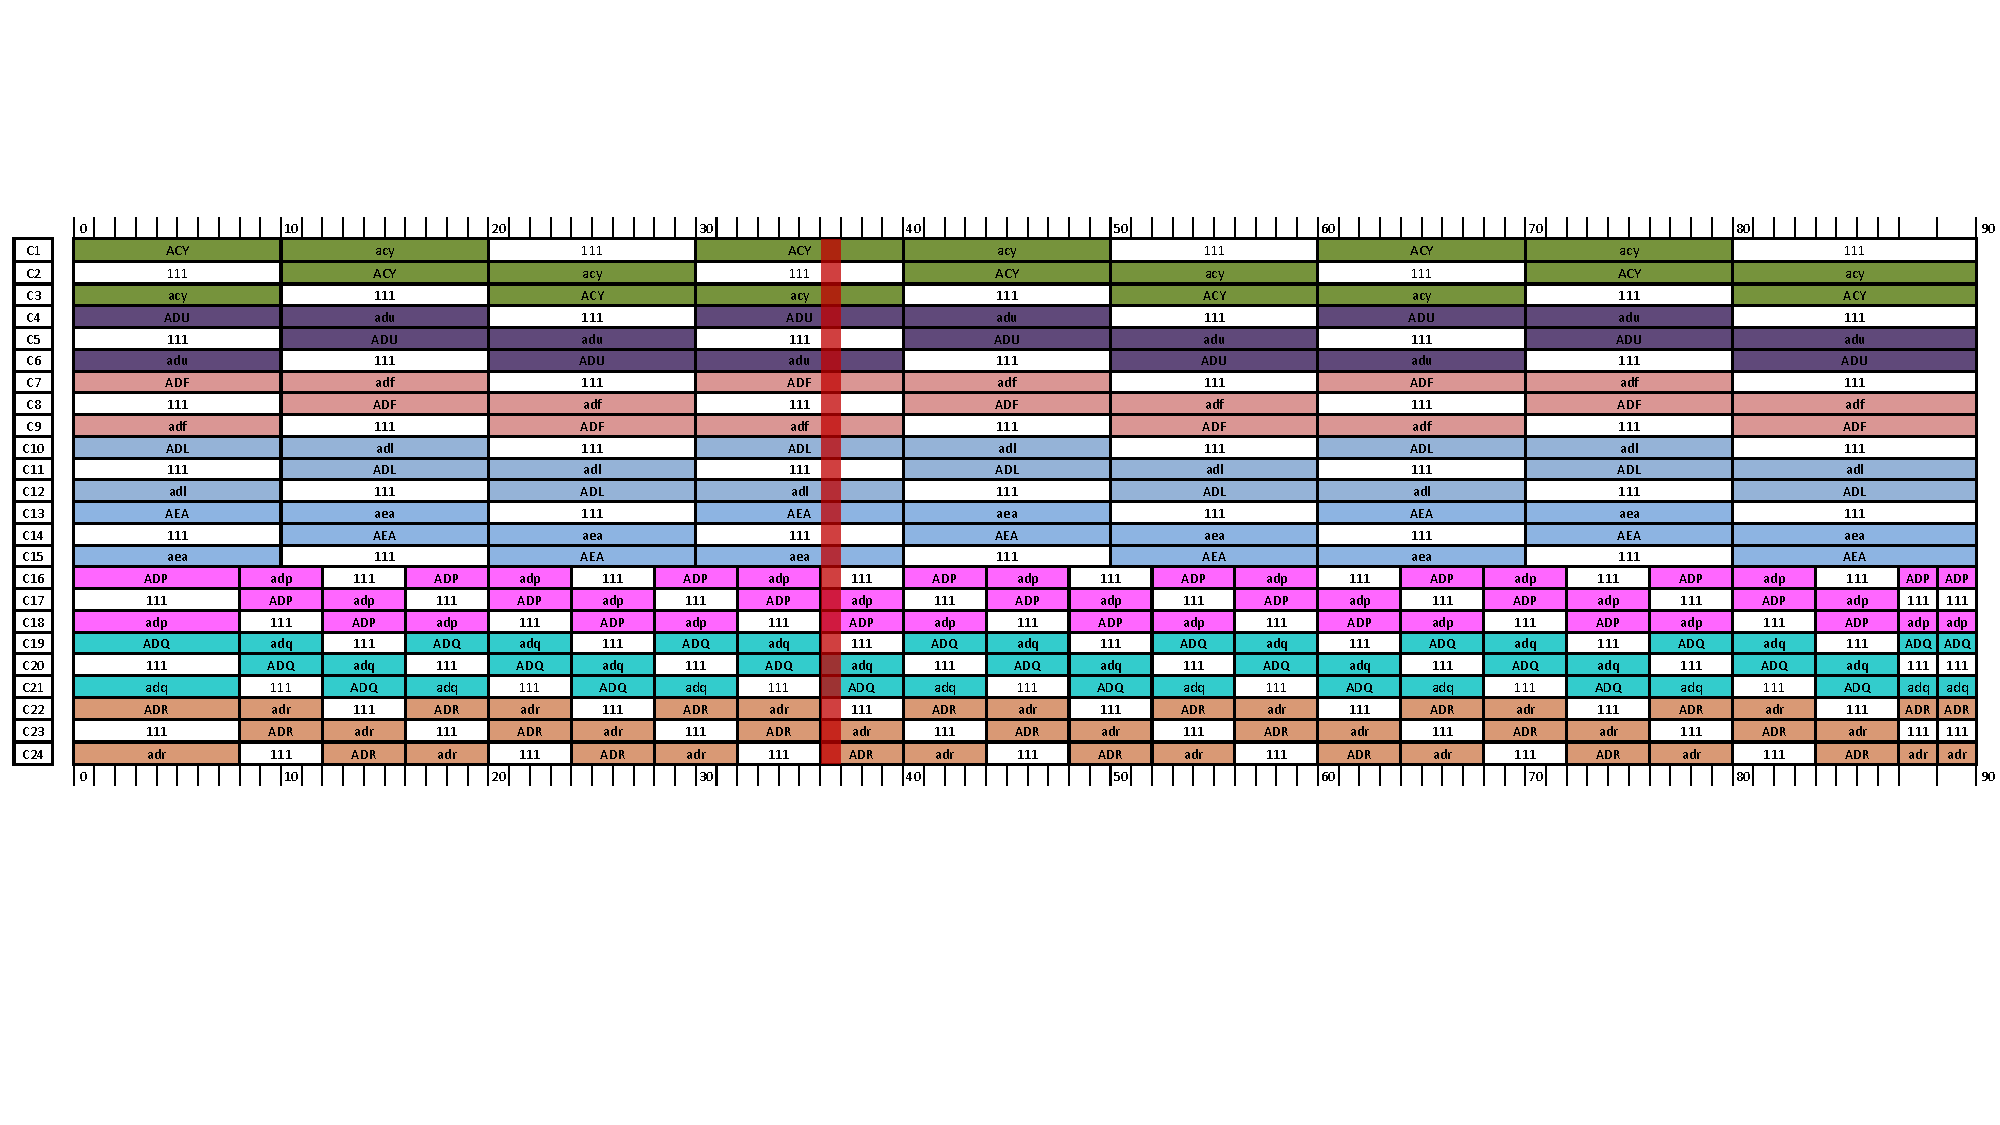
\includegraphics[width=\linewidth]{1-solucion-inicial-caso1}
	\caption{Aspecto visual de la planificación inicial del caso 1}
	\label{fig:5:solucion-inicial-caso1}
\end{figure}

\begin{figure}
	\centering
	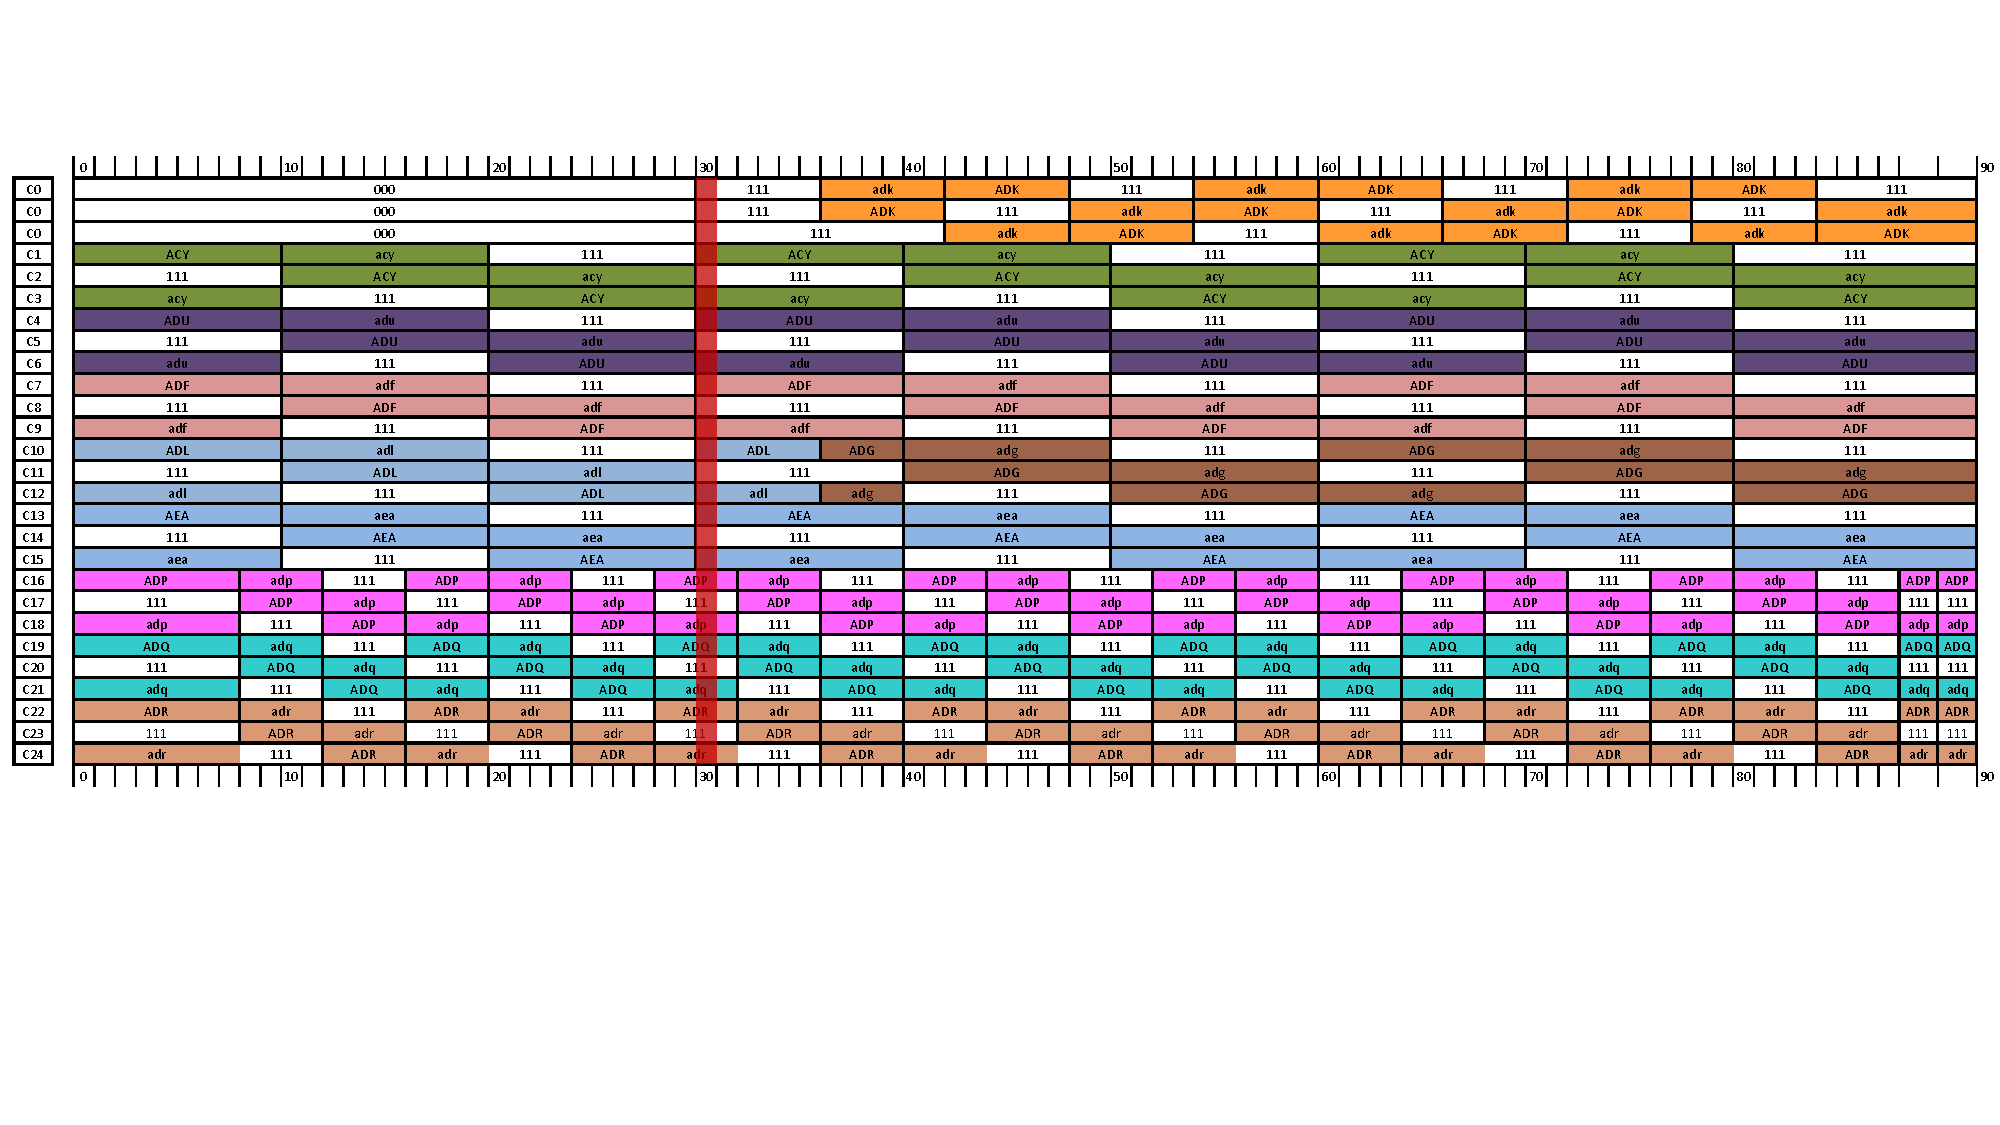
\includegraphics[width=\linewidth]{2-solucion-fase1-caso1}
	\caption{Aspecto visual de la solución inicial del caso 1, obtenida como salida de la \faseuno{}}
	\label{fig:5:solucion-fase1-caso1}
\end{figure}

Por su parte, la \fasedos{} que emplea la metaheurística de VNS (véase la \autoref{fig:5:solucion-fase2-vns-caso1}) logra eliminar todos los controladores imaginarios y reducir los recursos empleados a los mismos que los iniciales. Sin embargo, el SA (véase la \autoref{fig:5:solucion-fase2-sa-caso1}) no lo logra, dando como resultado una solución que emplea 25 controladores, uno más que la inicial. Como hemos mencionado, este valor es crítico para el sistema y por ello repercute en un gran impacto en el fitness, logrando, el VNS, un fitness total de $0.9718$ frente al $0.7117$ del SA. 

\begin{figure}
	\centering
	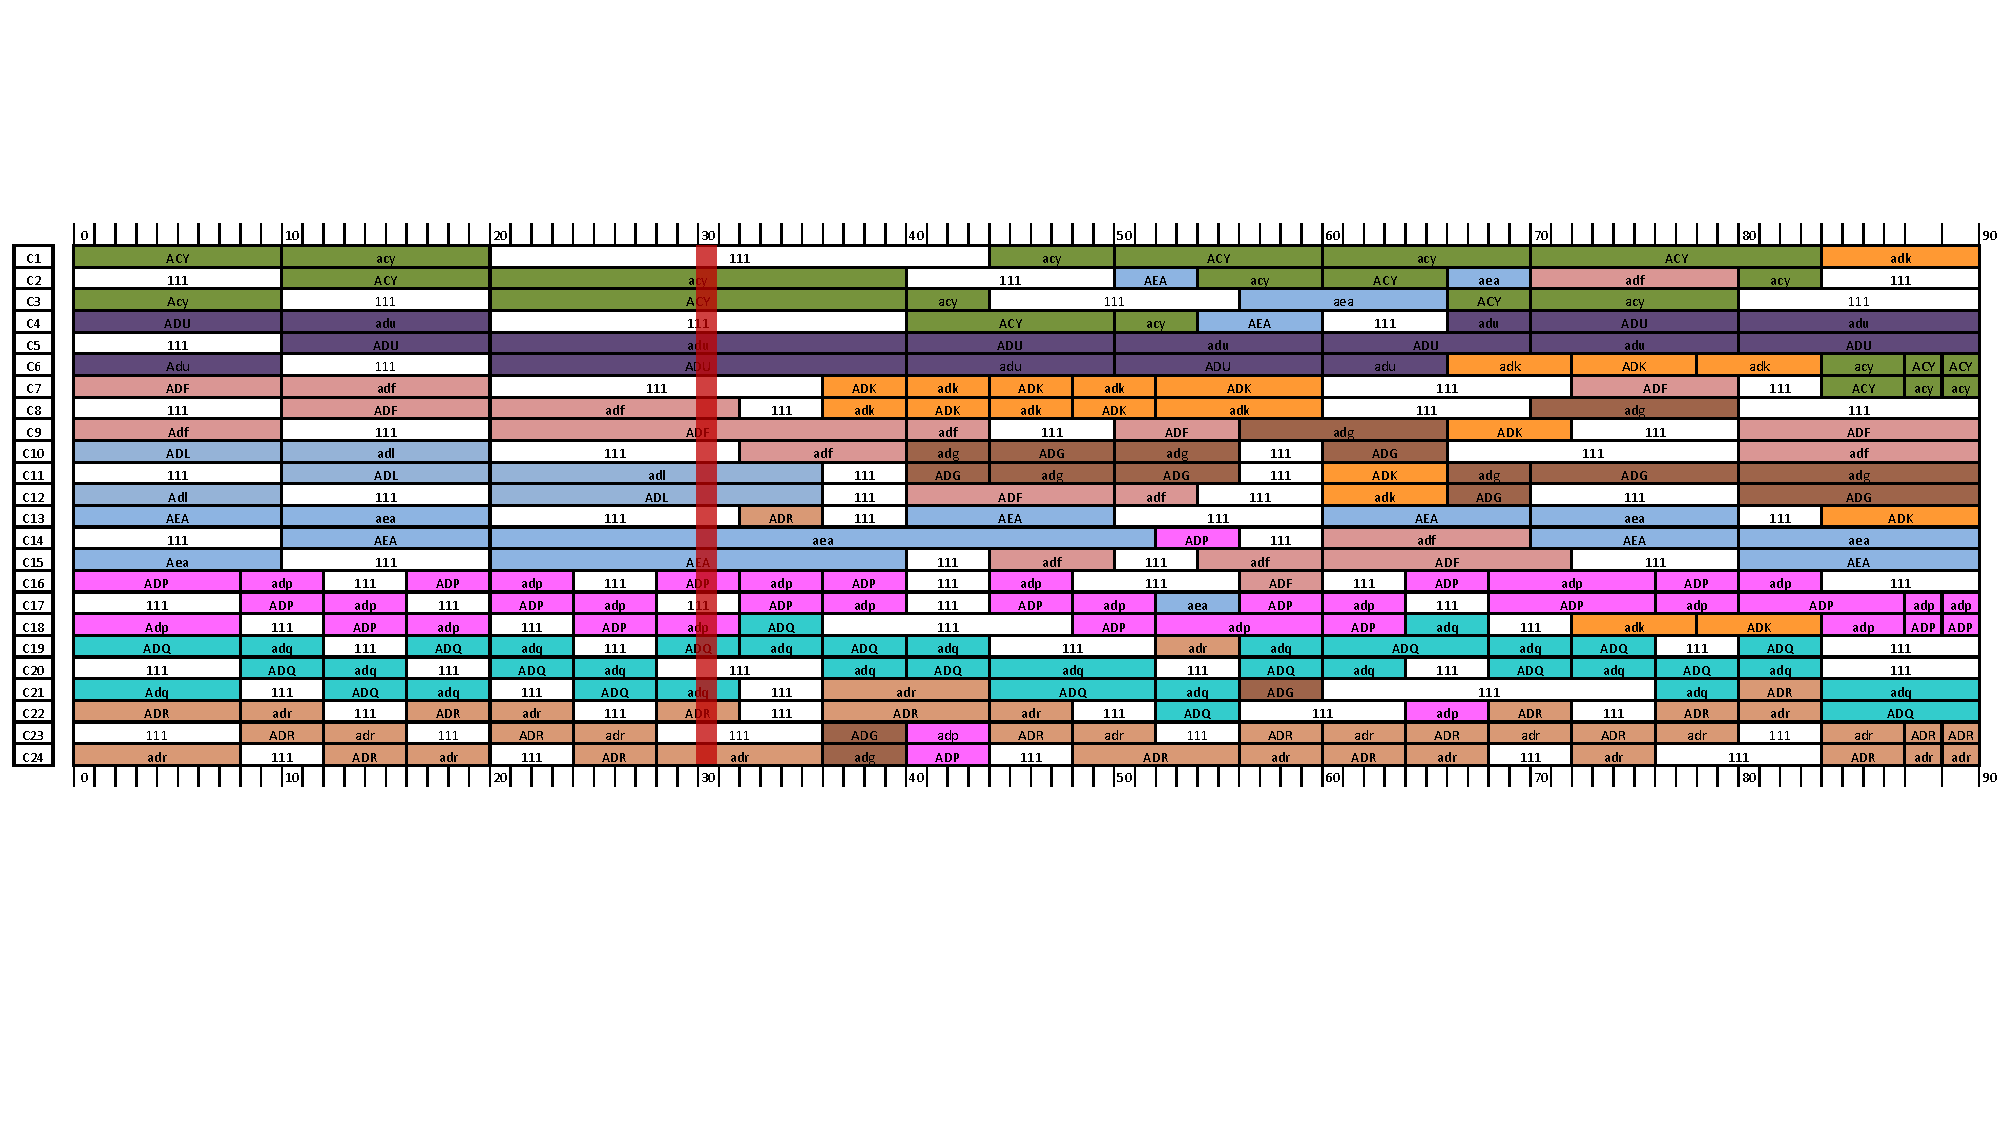
\includegraphics[width=\linewidth]{3-solucion-fase2-VNS-caso1}
	\caption{Aspecto visual de la solución final del sistema para el caso 1, empleando para la \fasedos{} la metaheurística VNS}
	\label{fig:5:solucion-fase2-vns-caso1}
\end{figure}

\begin{figure} 
	\centering
	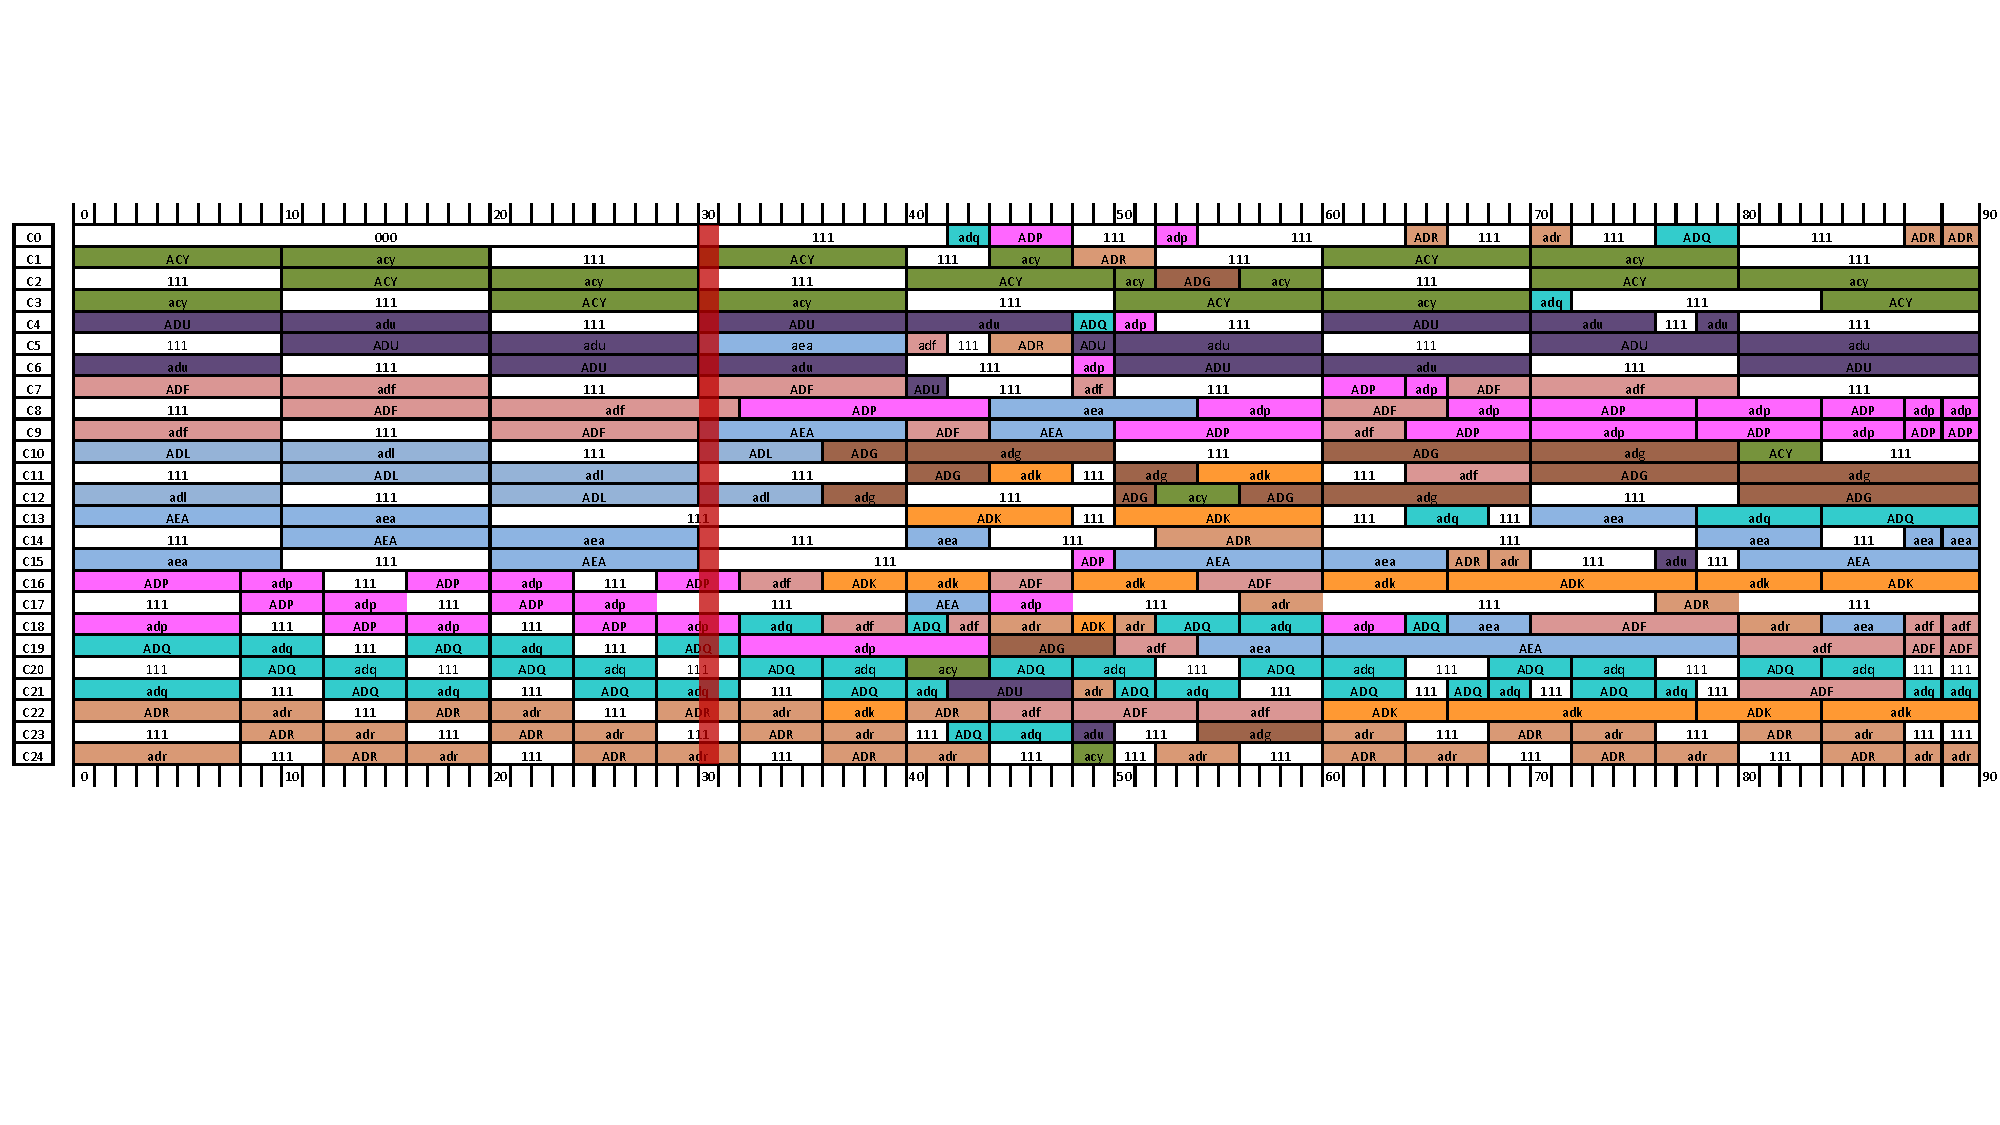
\includegraphics[width=\linewidth]{3-solucion-fase2-SA-caso1}
	\caption{Aspecto visual de la solución final del sistema para el caso 1, empleando para la \fasedos{} la metaheurística SA}
	\label{fig:5:solucion-fase2-sa-caso1}
\end{figure}

En cuanto a restricciones (\ref{O2}), la solución de VNS pasa inicialmente de incumplir 3 veces la restricción \ref{RD:9:tiempo-min-trabajo-continuado}, pues los dos últimos slots asignados a los controladores C16, C19 y C22 son de trabajo, lo que hace un total de 10 minutos, cuando el tiempo de trabajo mínimo es de 15 minutos, que son 3 slots.
Al adaptar la planificación inicial al problema del caso 1, añadimos el incumplimiento de una restricción más: \ref{RD:controlador-por-cada-turno}, pues existen 3 turnos sin controlador real asignado.
Por último, la solución final logra reparar los problemas relativos a ambas restricciones antes nombradas, sin embargo a costa de incumplir las restricciones \ref{R:5:max-trabajo-continuado} y \ref{RD:3:porcentaje-min-descanso}, que están relacionadas entre sí, en 6 y 4 ocasiones respectivamente: para la solución que propone el sistema, algunos controladores deberán de trabajar más tiempo del adecuado y por consiguiente, descansar menos tiempo, algunos incluso por debajo del mínimo de tiempo total de la jornada.

Respecto al objetivo \ref{O3} y el objetivo \ref{O4}, el VNS parece que lo afronta mejor. Podemos apreciarlo visualmente: el momento del cambio es más homogéneo y la similitud a las plantillas es mayor en el caso del VNS.

\subsubsection{Análisis del Caso 7}

En el caso 7 obtenemos unas soluciones peores que en el caso anterior, algo comprensible teniendo en cuenta la dificultad del caso (véase la \autoref{sec:5:def-casos}), pero muy superiores pese a ello, a las del SA. 

La planificación inicial de la que partimos consta de un total de 25 controladores. 
En la \faseuno{} se producen tres incidencias: varios cambios de sectorización, una baja y un alta.
La forma en la que las sectorizaciones cambian se encuentra representada en la \autoref{fig:5:esquema-sectorizacion-caso7}, que agrupa por colores aquellos sectores afines. 
Recuérdese que no es la misma sectorización 3A para el núcleo Ruta Este que para el Oeste. 

En la \autoref{fig:5:solucion-inicial-caso7} puede observarse el resultado del proceso que describiremos a continuación.

Por ejemplo, el núcleo Oeste pasa de una configuración 5A a una 5C a partir del slot 20, cerrándose cuatro sectores (ADL, ADP, ADQ y ADR) y abriéndose otros cuatro (ADH, ADI, ADM y ADN); uno de ellos permanece estático (AEA). 
A la hora de sustituir por afinidades (véase la \autoref{sec:3:fase1-paso1}), la heurística implementada sustituirá ADL por ADH, ADP por ADM y ADR por ADN, tal y como muestran ambas figuras. Por lo tanto, no es necesario añadir plantillas para estos sectores. Por último, al no haber afinidades entre los dos sectores que faltan, se ha de eliminar, durante el periodo de tiempo pertinente, la presencia del sector ADQ en la solución y añadir una nueva plantilla con tres controladores imaginarios para el sector ADI.

\begin{figure}
	\centering
	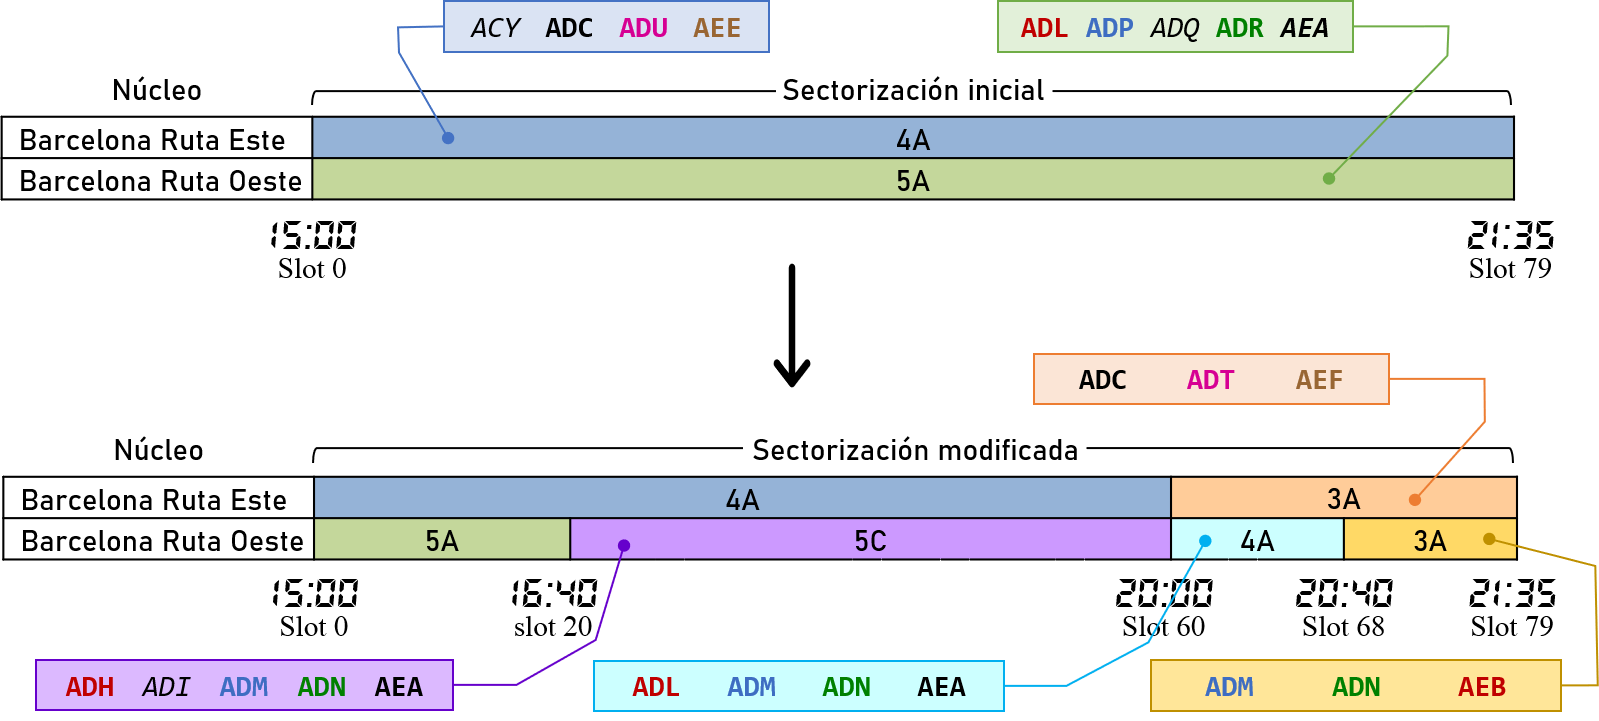
\includegraphics[width=\linewidth]{esquema-sectorizacion-caso7}
	\caption{Diagrama que representa la sectorización inicial y la modificada para el caso 7}
	\label{fig:5:esquema-sectorizacion-caso7}
\end{figure}

Por otro lado, para gestionar la baja del controlador C23 que se produce en el slot 42, se mueve toda su carga a partir de ese instante a un nuevo controlador imaginario, marcando ese intervalo de tiempo en C23 como inamovible para la \fasedos{} (mediante el ``000'').
Para gestionar el alta del nuevo controlador C26, se añade al final, y solo se permite que la \fasedos{} añada carga a partir del slot 60, que es cuando se produce el alta.

\begin{figure}
	\centering
	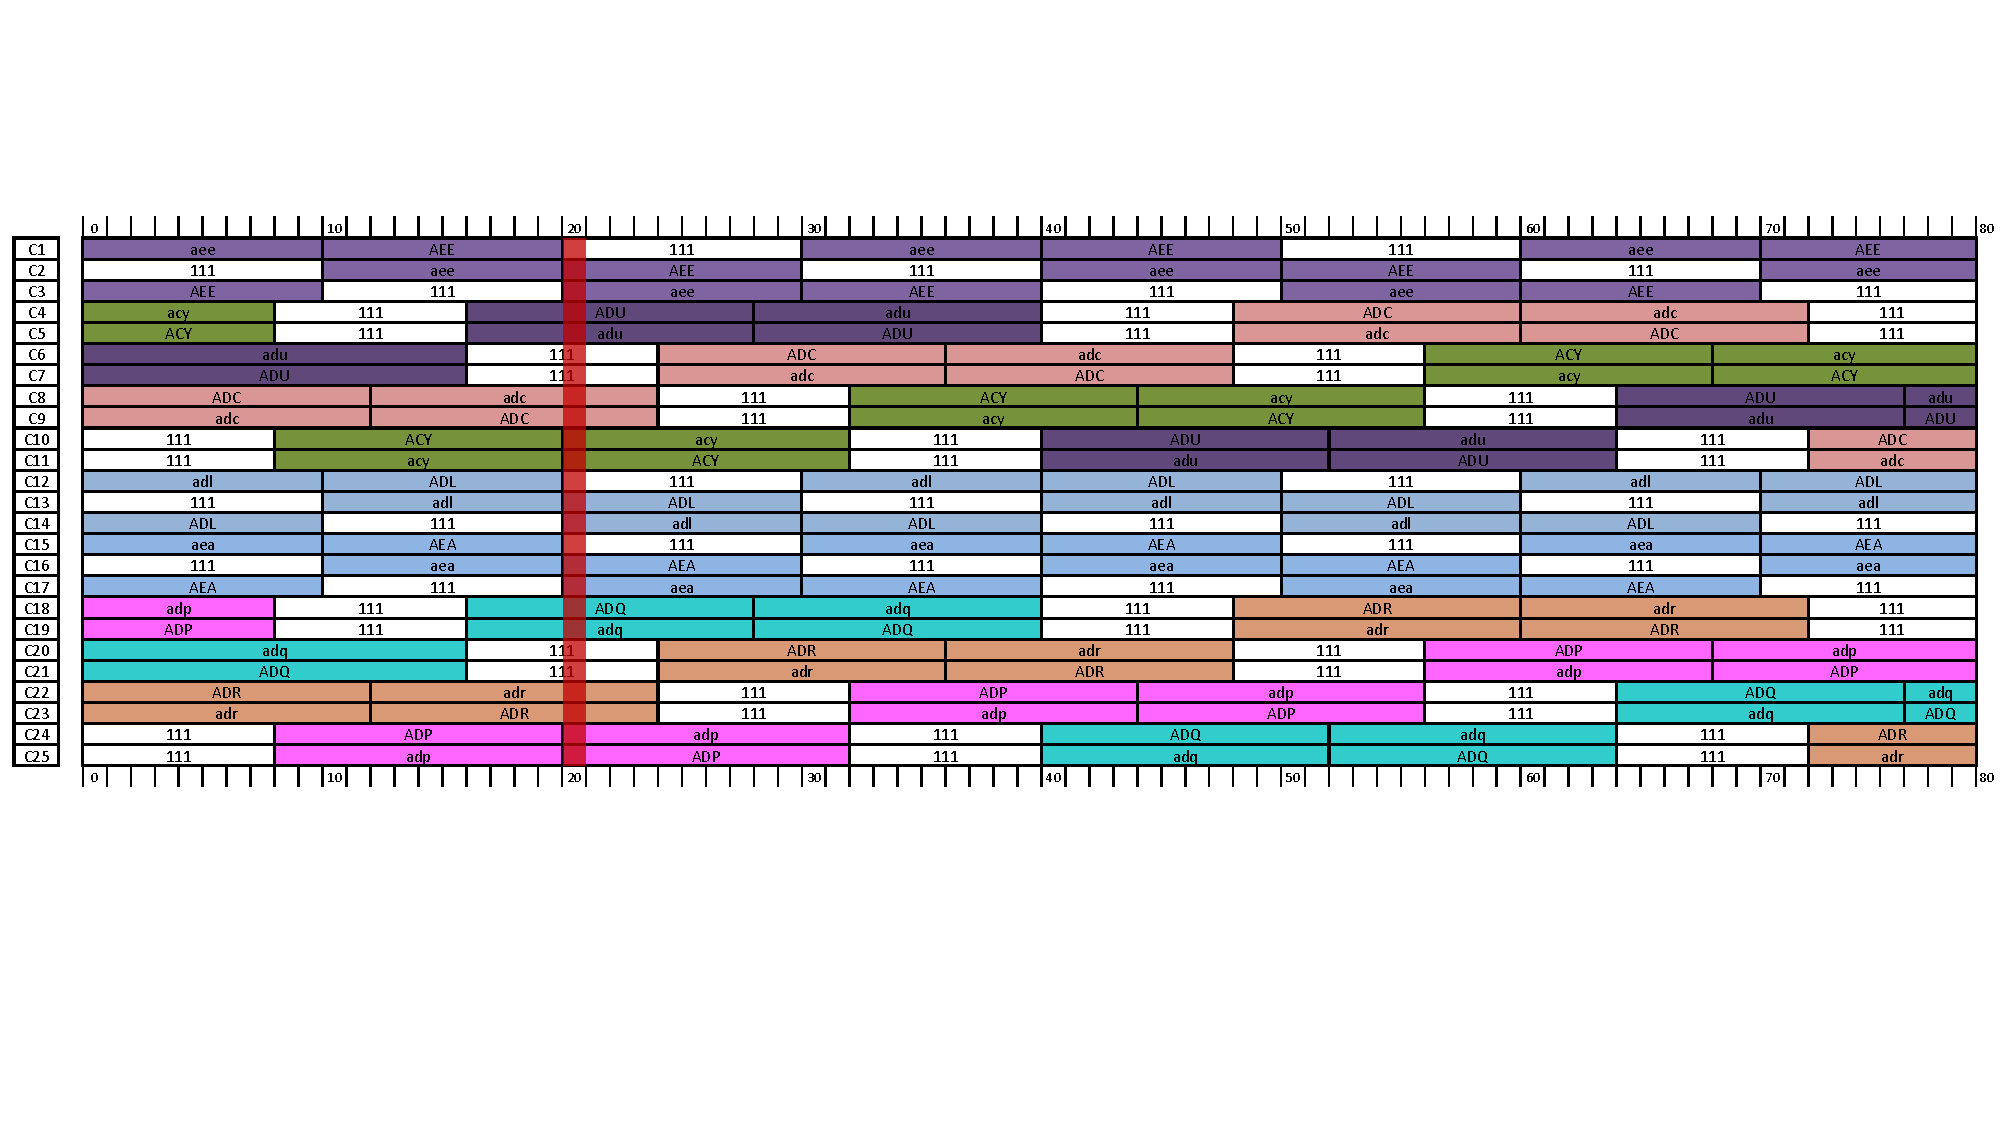
\includegraphics[width=\linewidth]{1-solucion-inicial-caso7}
	\caption{Aspecto visual de la planificación inicial del caso 7}
	\label{fig:5:solucion-inicial-caso7}
\end{figure}

\begin{figure}
	\centering
	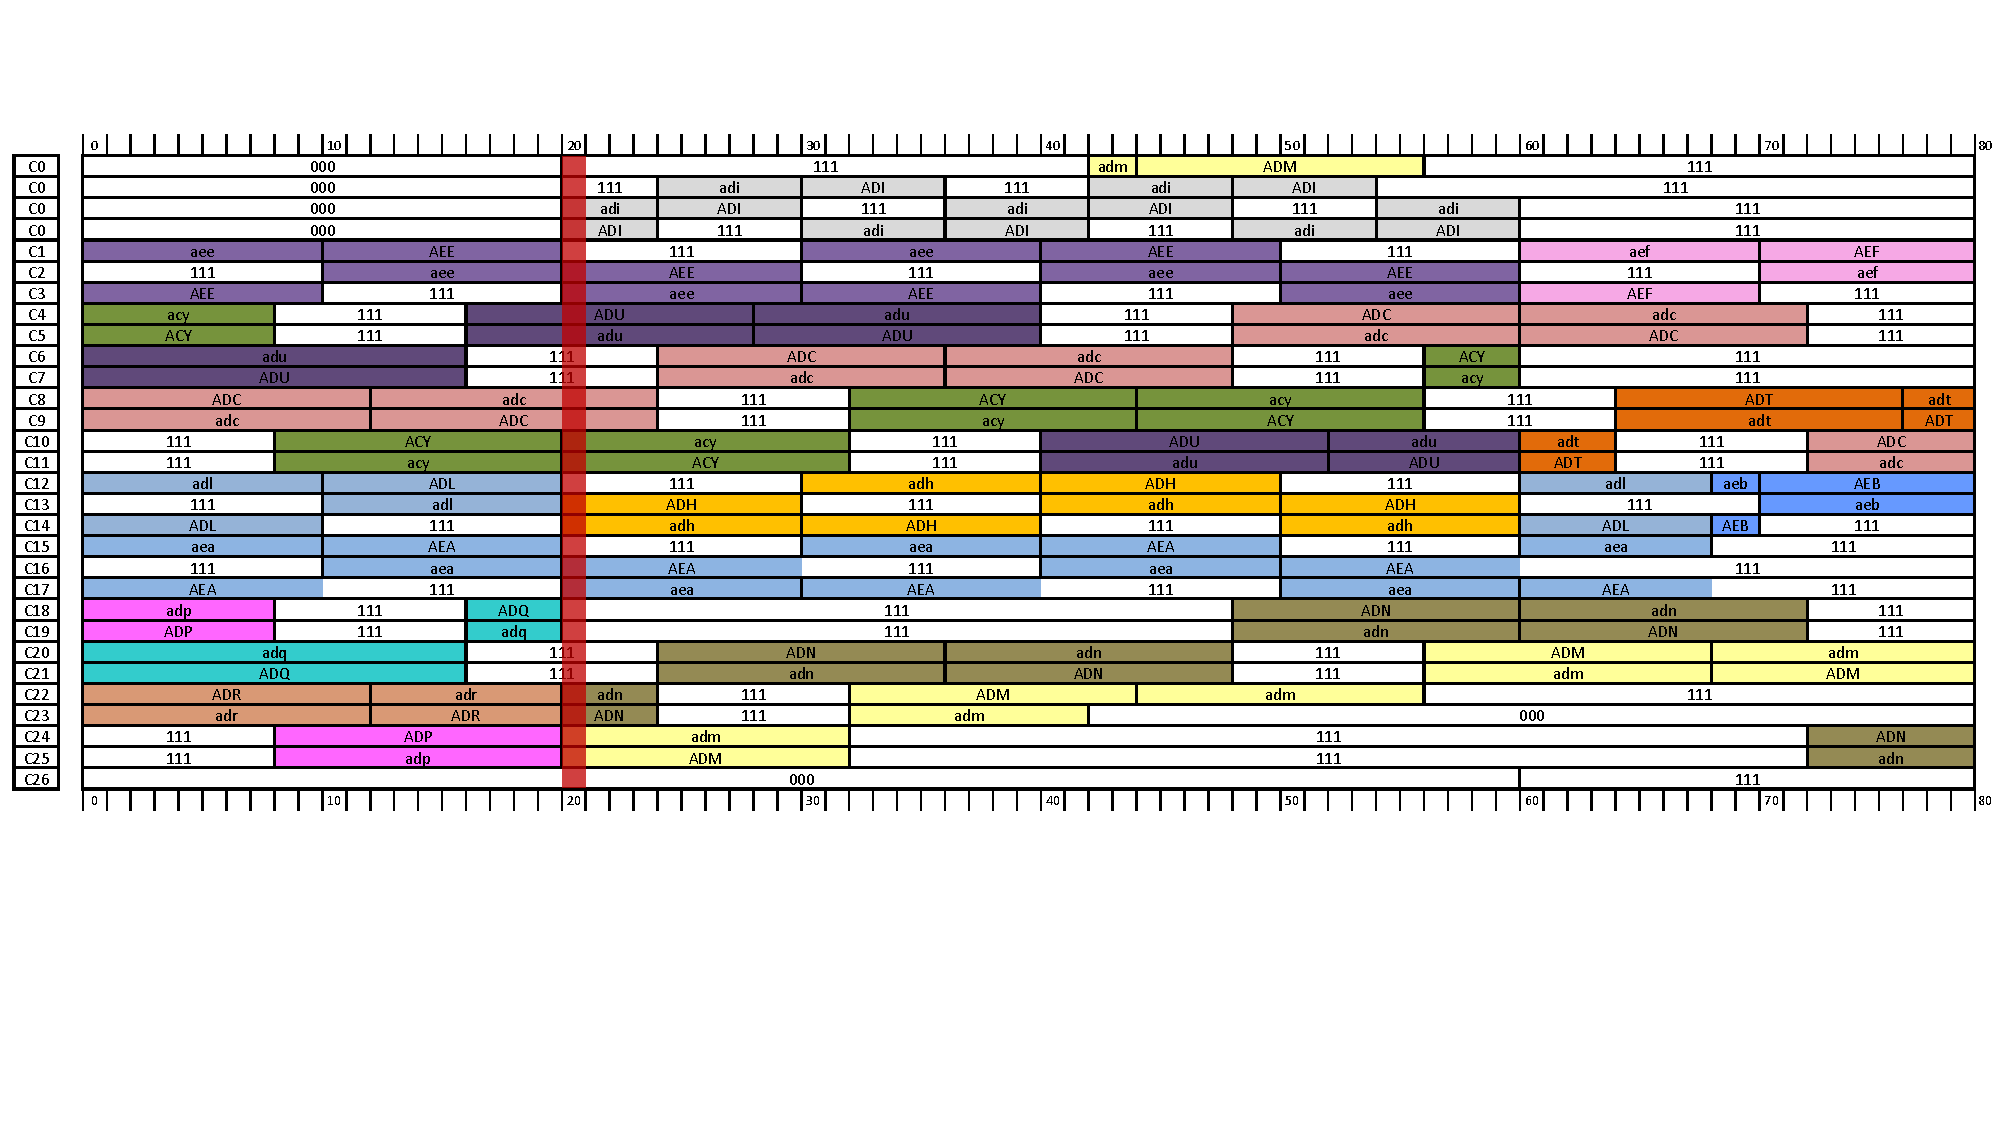
\includegraphics[width=\linewidth]{2-solucion-fase1-caso7}
	\caption{Aspecto visual de la solución inicial del caso 7, obtenida como salida de la \faseuno{}}
	\label{fig:5:solucion-fase1-caso7}
\end{figure}

De esta forma, la solución inicial que ofrece la \faseuno{} consta de un total de 28 controladores, de los cuales cuatro son imaginarios (véase la \autoref{fig:5:solucion-inicial-caso7}). La \fasedos{} toma dicha planificación y la logra reducir a 26 controladores en su solución final, eliminando todos los imaginarios (véase la \autoref{fig:5:solucion-fase2-vns-caso7}). Una diferencia muy grande respecto al SA, que ni siquiera logra reducir un solo controlador (véase la \autoref{fig:5:solucion-fase2-sa-caso7}). Por ello, la diferencia de valor total de la solución es muy grande: el SA obtiene una media de $0.6146$ mientras que el VNS logra la cifra de $0.9335$.

\begin{figure}
	\centering
	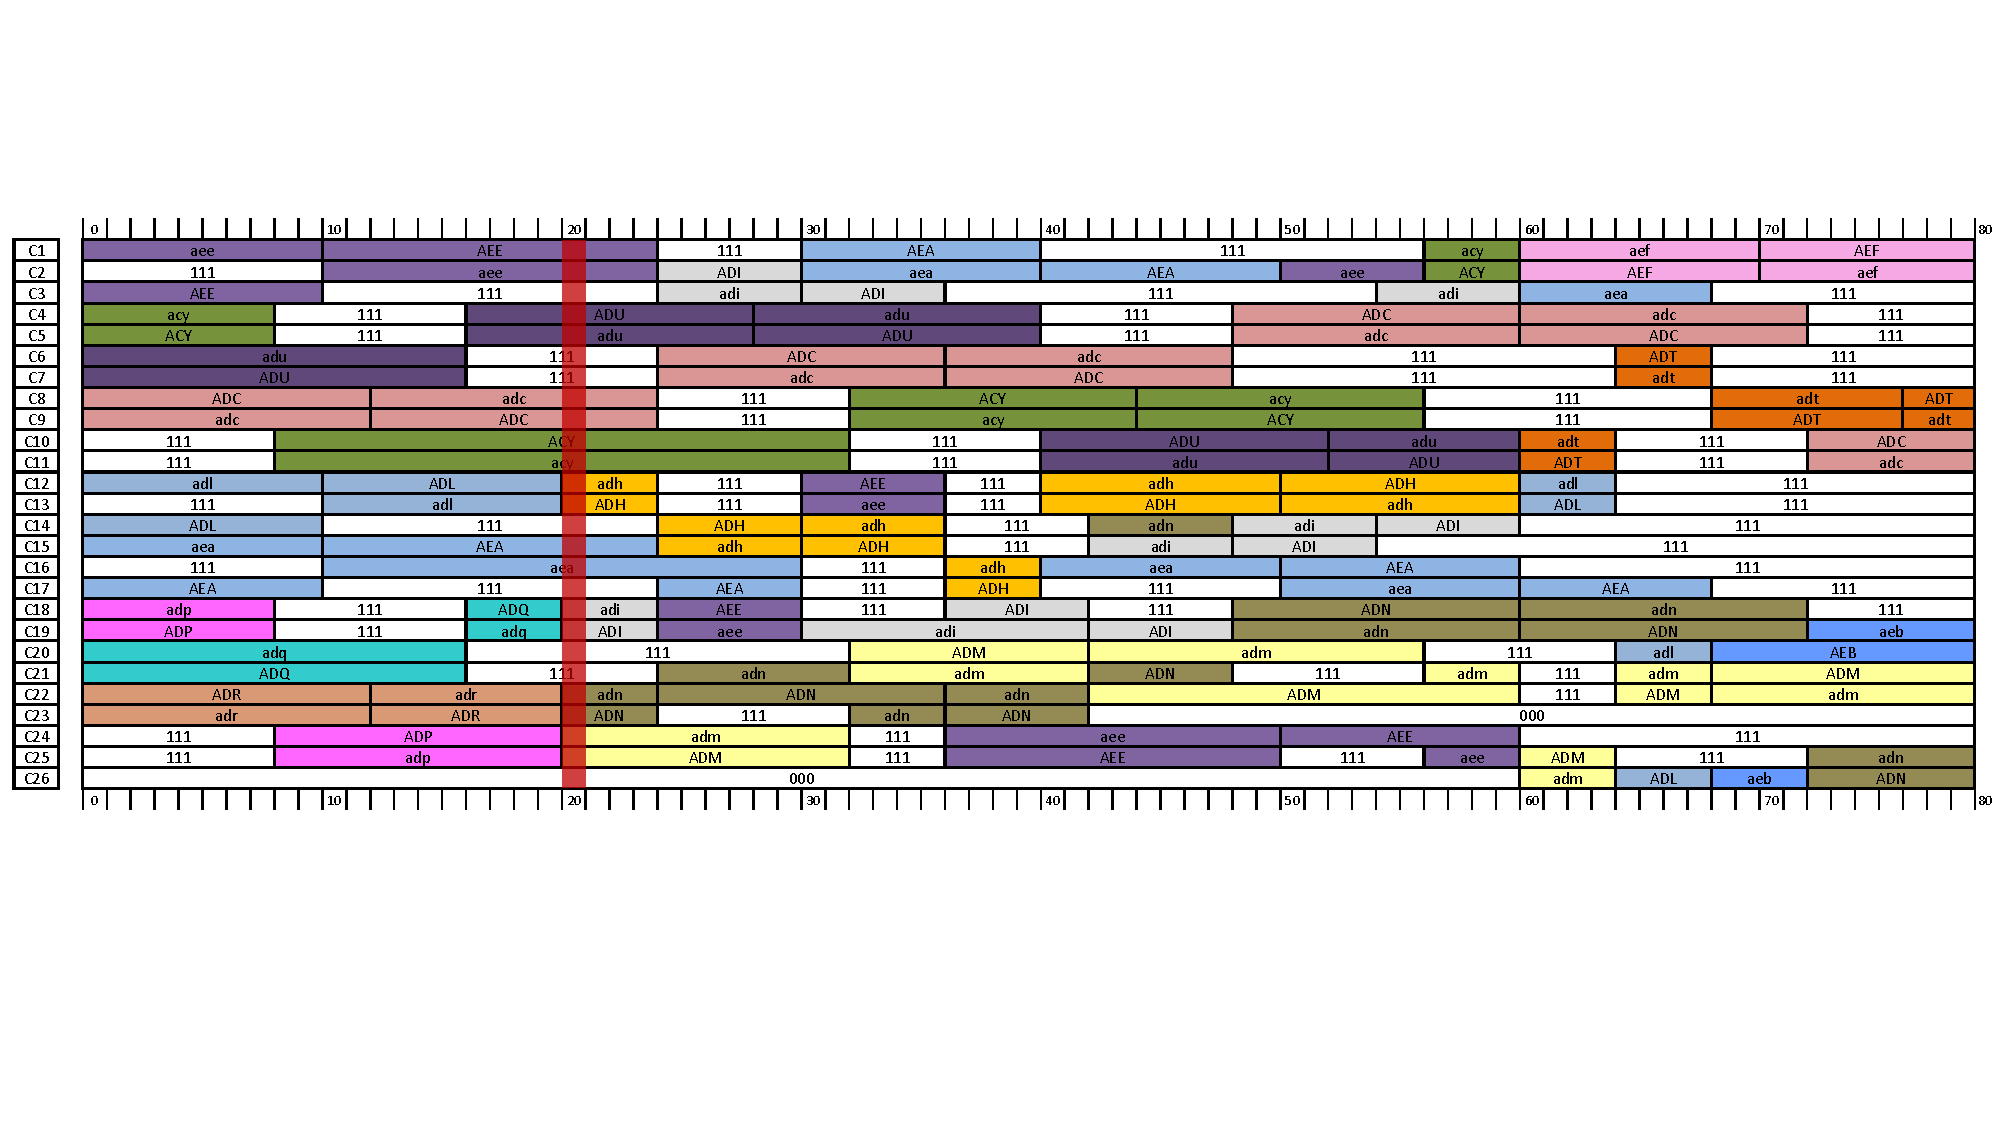
\includegraphics[width=\linewidth]{3-solucion-fase2-VNS-caso7}
	\caption{Aspecto visual de la solución final del sistema para el caso 7, empleando para la \fasedos{} la metaheurística VNS}
	\label{fig:5:solucion-fase2-vns-caso7}
\end{figure}

\begin{figure}
	\centering
	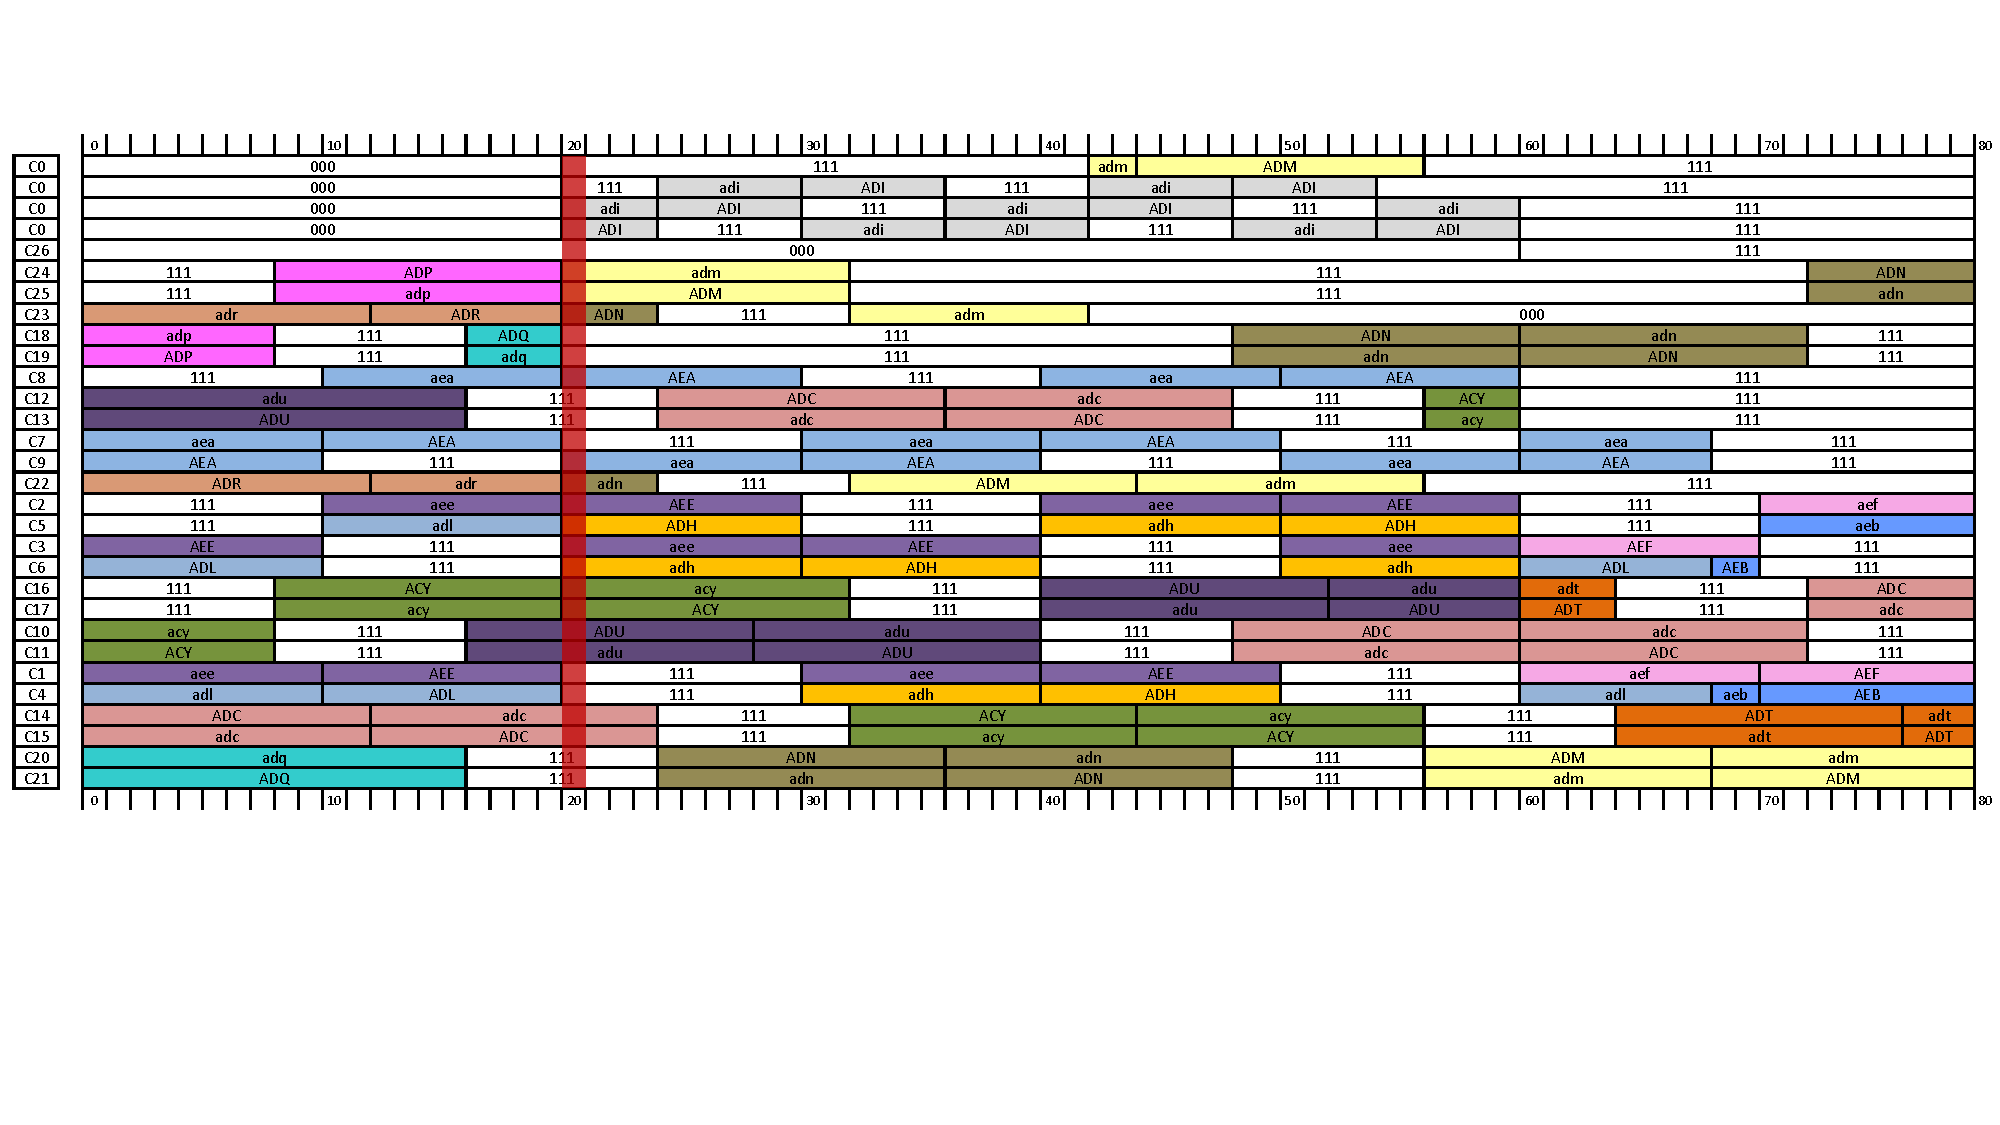
\includegraphics[width=\linewidth]{3-solucion-fase2-SA-caso7}
	\caption{Aspecto visual de la solución final del sistema para el caso 7, empleando para la \fasedos{} la metaheurística SA}
	\label{fig:5:solucion-fase2-sa-caso7}
\end{figure}

En cuanto a los demás objetivos, VNS es superior aunque similar tanto para el número de restricciones incumplidas \ref{O2} como para la semejanza a las plantillas \ref{O4}, aunque observamos resultados notablemente mejor, en media, para el \ref{O3}: la minimización del número de cambios en sala en el momento de la incidencia.

\subsubsection{Análisis del Caso 3}

Por último, parece importante destacar también las limitaciones del sistema, que se ponen de manifiesto notablemente en el caso 3, donde hay muy pocos huecos donde poder mover carga. 

El caso 3 consta de la incidencia de una baja del controlador C23 en el slot 24. No se producen altas, por lo que se necesita de un controlador imaginario. Y ese es el mayor inconveniente, pues eliminarlo será una tarea muy difícil de resolver teniendo en cuenta el poco margen de movimientos que tiene. 

Además, debido al orden establecido de importancia, los demás objetivos no será tomados tan en cuenta, especialmente el \ref{O4}, que trata de asemejar lo máximo posible la solución con las plantillas, puesto que su funcionamiento contradice al del objetivo \ref{O1}, en el sentido de que este último precisa de la ordenación de los turnos según la carga de trabajo asignada, mientras que \ref{O4} necesita que los turnos estén en el orden inicial, para poder comparar con la forma de las plantillas. % TODO: poner esto también en el capítulo 3!!!

Debido a ello, las soluciones alcanzadas son de peor calidad. Y es que el caso 3 es el que peor desempeña el sistema, aumentando el número de restricciones incumplidas respecto a la solución inicial y asignando una sobrecarga a la mayoría controladores, con el fin de encontrar hueco para eliminar el controlador imaginario, algo que nunca llega a producirse.

\NOTE{HE DETECTADO UN ERROR EN LOS FICHEROS ENVIADOS POR CRIDA: EL MOMENTO DEL CAMBIO DEL CASO 3 ES POSTERIOR A LA DE LA INCIDENCIA POR LO QUE NO PUEDE MOVER PARTE DE ESA CARGA Y POR ESO NO PUEDE ELIMINAR EL CONTROLADOR. NECESITO DATOS DEL SA CON EL MOMENTO DEL CAMBIO A LAS 9:30 EN VEZ DE A LAS 10!!!}

\subsection{Otros experimentos}

\subsubsection{Comparativa \textit{First Improvement} y \textit{Best Improvement}}

En el \autoref{capitulo:3} describimos las alternativas de metodología y parámetros barajadas en el TFM y por qué fueron elegidas finalmente las empleadas. Una de esas alternativas se trata del comportamiento de la búsqueda local, pudiendo ser \textit{First Improvement} y \textit{Best Improvement}. La segunda, no puede ser aplicada en este problema debido a que no podemos generar todas las posibles soluciones (para quedarnos con la mejor), por lo que se propuso una opción híbrida que precisaba de dos nuevos parámetros al sistema: el número máximo de iteraciones sin mejora para la búsqueda local y el porcentaje mínimo de mejoría para la búsqueda local.

Un experimento interesante puede ser una comparativa entre ambos comportamientos, que puede verse la \autoref{fig:5:first-vs-bestiteracioncaso1}, que representa gráficamente el desempeño medio en cada iteración para el caso 1, que emplea un \textit{VND}, que es únicamente determinista, por lo que tan solo emplea la búsqueda local como medio de búsqueda dentro del entorno. Se ha llamado al comportamiento híbrido como simplemente \textit{Best Improvement} por ser una adaptación de este.

\begin{figure}
	\centering
	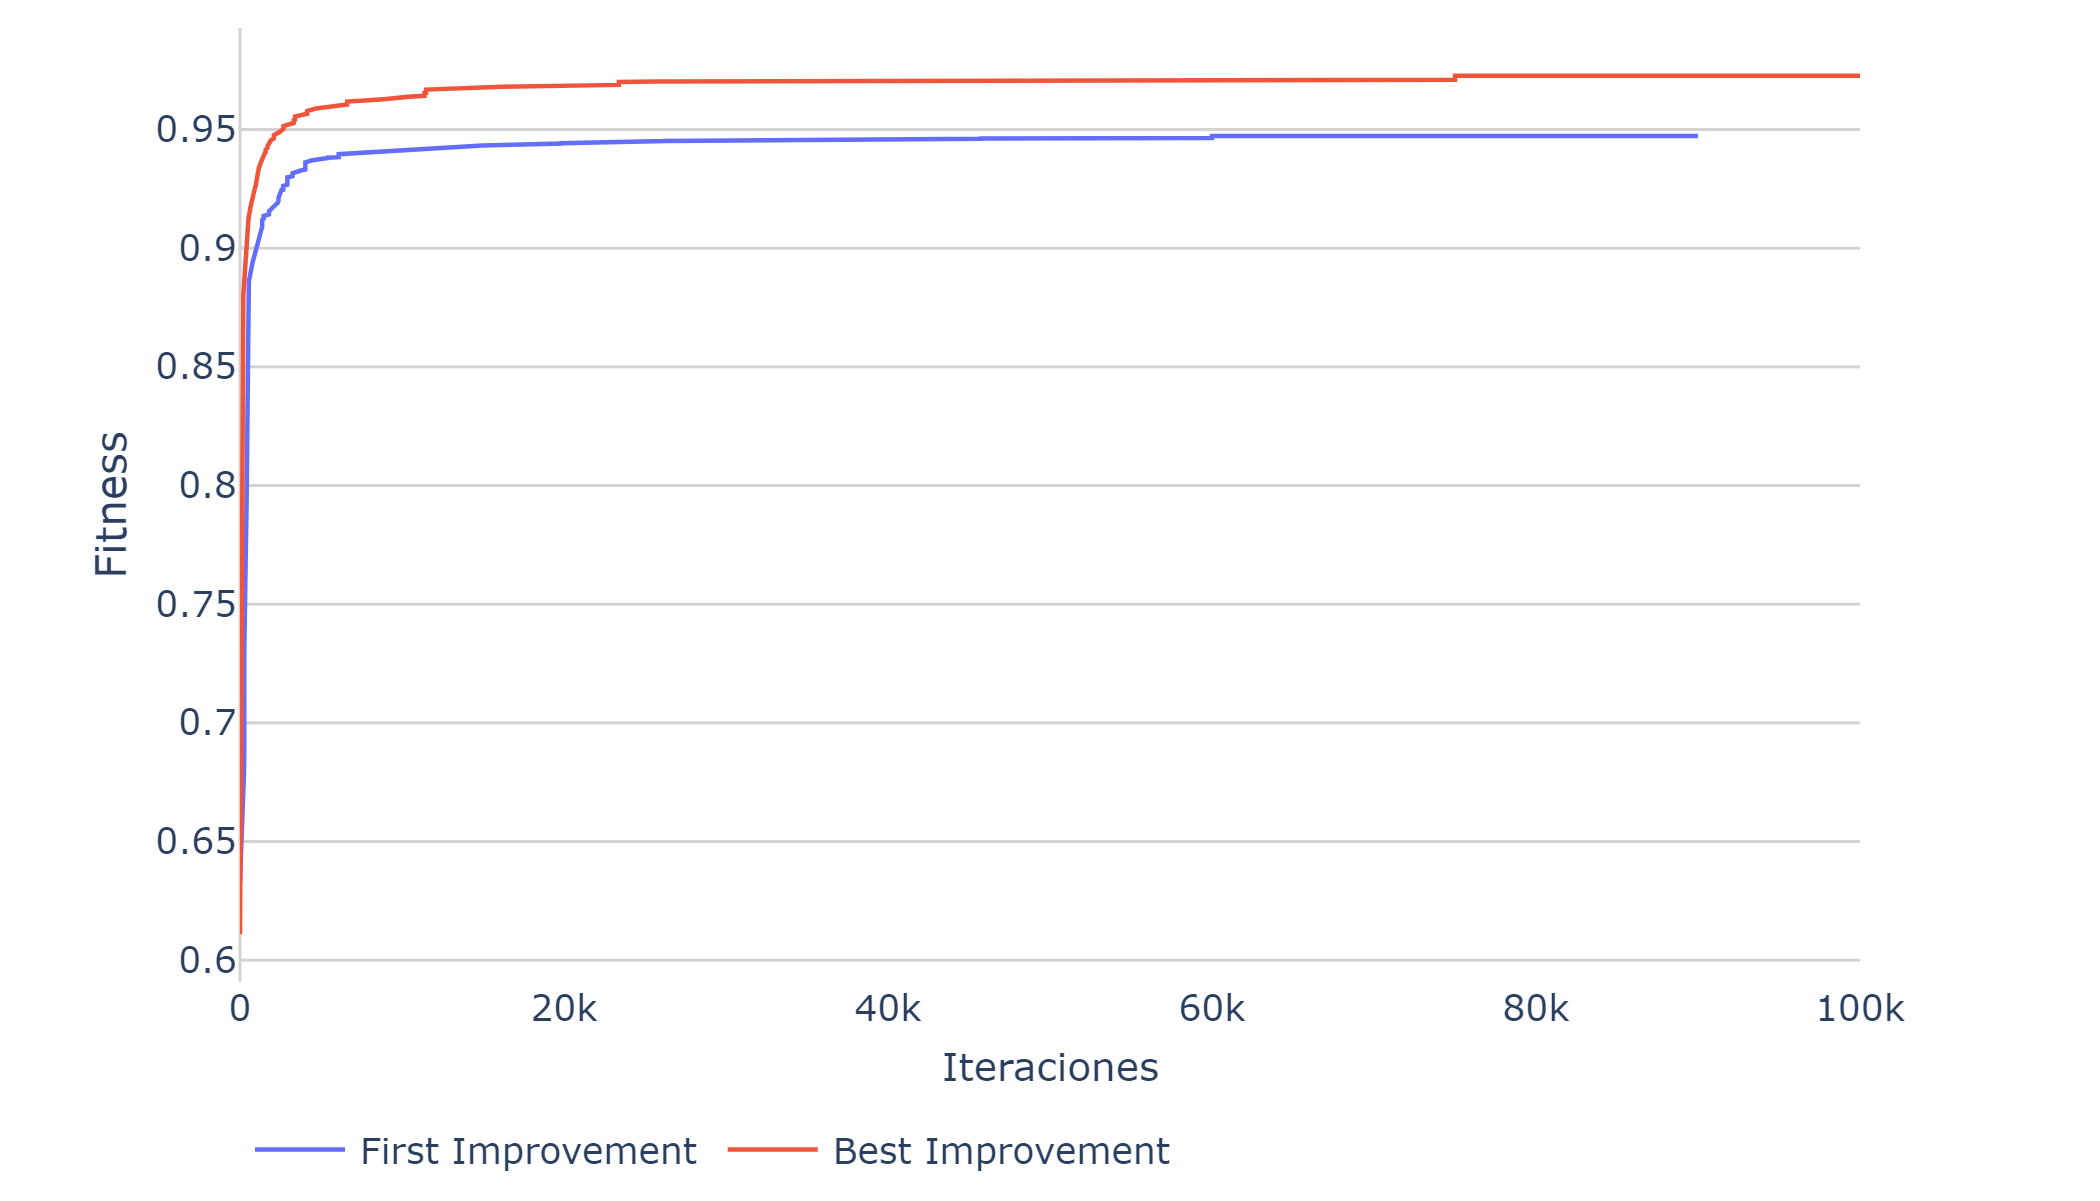
\includegraphics[width=\linewidth]{First-vs-best_iteracion_Caso1}
	\caption{Gráfica comparativa del desempeño del sistema para el caso 1, empleando los dos posibles comportamientos de la búsqueda local}
	\label{fig:5:first-vs-bestiteracioncaso1}
\end{figure}

Podemos observar cómo el comportamiento propuesto mejora sustancialmente el desempeño final del algoritmo.